\documentclass{ufabc}

\usepackage{amscd}
\usepackage{amsfonts}
\usepackage{amssymb}
\usepackage{epsf}
\usepackage{graphicx}
\usepackage{algorithm}
\usepackage{algpseudocode}
\usepackage{pifont}
\usepackage{indentfirst}
\usepackage{amsmath}
\usepackage[only,ninrm,elvrm,twlrm,fivrm,sixrm,sevrm,egtrm,egtit,tenrm,tenit,twlit,frtnrm]{rawfonts}
\usepackage{titlesec}

\instituicao{Universidade Federal do ABC\\Centro de Matem�tica, Computa��o e Cogni��o (CMCC)}
\curso{Curso de P�s-Gradua��o}{Ci�ncia da Computa��o}{Mestre}
\titulo{Agentes inteligentes para batalhas Pok�mon}
\autor{Jonathan Ohara}{de Araujo}
\orientador{Orientador: Prof. Dr. Fabr�cio Olivetti de Fran�a}
\coordenador{Prof. Dr. Jo�o Paulo Gois}	
\documento{Trabalho}
\convidados{Prof. Dr. Fabr�cio Olivetti de Fran�a}{Prof.Dr. Jo�o Paulo Gois}{Prof.Dr. Andr� Luiz Brand�o}{Prof.Dr. Denise Hideko Goya (Suplente)}
	
\date{03}{2017}

\setcounter{secnumdepth}{5}
\MakeRobust{\Call}

% novos comandos para qualificacao
\newcommand{\kCC}{\emph{kCC}}
\newcommand{\kCH} {\emph{kCH}}
\newcommand{\uCC}{\emph{1CC}}
\newcommand{\uCH} {\emph{1CH}}
\newcommand{\dCC}{\emph{2CC}}
\newcommand{\dCH} {\emph{2CH}}
\newcommand{\PTH}{\mathcal{P}}
\newcommand{\Tau}{\mathcal{T}}
\newcommand{\NP}{{\rm NP}}


\begin{document}
	\maketitle

	\pagenumbering{roman}
	
	\begin{resumo}
Esse trabalho explora a cria��o de agentes inteligentes competitivos em um ambiente onde dezenas de milhares de jogadores humanos competem diariamente para melhorar sua coloca��o no sistema de ranqueamento do jogo Pok�mon Showdown.

Escolher o melhor algoritmo e a melhor forma de aprendizado para jogar contra humanos � um dos grandes desafios desse trabalho. Outro importante aspecto que o agente precisa se adaptar � a grande variedade de composi��es de times e Pok�mons que o agente e o seu advers�rio pode montar.

Para obter a melhor flexibilidade o agente ser� submetido somente a batalhas rand�micas onde as composi��o das equipes s�o todas aleat�rias, e a avalia��o de performance do agente ser� feita atrav�s do sistema de ranqueamento do pr�prio jogo.
\end{resumo}
	\begin{resumoingles}

To Do.

\end{resumoingles}	

	\tableofcontents
	
	\listoffigures
	
	\listoftables

	\newpage
	
	\pagenumbering{arabic}

	\chapter{Introdu��o}
\label{cap:introducao}

\section{Motiva��o}
\label{sec:motivacao}

Existem diversas finalidades para cria��o de agentes inteligentes para jogos. Podemos enumerar algumas como: adapta��o a diferentes tipos de jogador, gerar diferentes experi�ncias em cada nova partida, gerar grandes desafios entre outras.

Esse trabalho explora a cria��o de agentes inteligentes que compitam com jogadores humanos no sistema de batalhas \textit{Pok�mon} no ambiente \textit{Pok�mon Showdown}.

Um dos grandes desafios na cria��o desses agentes � a adaptabilidade e a competitividade. Diferentes de jogos como xadrez, damas, reversi e outros jogos de tabuleiro, em batalhas \textit{Pok�mon} nada se sabe do advers�rio at� que comece o jogo, ou seja, invalidando qualquer tipo de t�cnica prevendo poss�veis movimentos antes do jogo come�ar j� que cada time pode ser montado de uma infinidade de modos diferentes. Para acentuar ainda mais essas proprieaddes os agentes ir�o treinar e competir no modo rand�mico, nesse modo a escolha do seu time assim como de seu advers�rio � feito pelo pr�prio sistema do jogo.

Por causa da caracter�stica de desconhecimento do time advers�rio, a utiliza��o de t�cnicas de cria��o de �rvores de poss�veis jogadas do advers�rio � bastante prejudicada, pois o agente precisaria predizer os poss�veis \textit{Pok�mons} advers�rios assim como suas caracter�sticas, assim dificultando a utiliza��o da t�cnica que ficou famosa pelo sistema \textit{Deep Blue} que segundo o trabalho \textit{Deep Blue System Overview} \cite{deepblue1} "O \textit{Deep Blue} � um massivo sistema paralelo para realiza��o de busca em �rvores de jogos de xadrez".

\section{Objetivos}
\label{sec:objetivos}
O Objetivo desse trabalho � o desenvolvimento de agentes inteligentes que joguem e aprendam com milhares de jogadores humanos. Ser� implementada distintas t�cnicas para cria��o e aprendizado desses agentes. No decorrer do trabalho ser� sumarizado a evolu��o dos agentes no sistema de ranqueamento do jogo e, essa posi��o ser� confrontada com a quantidade de treinamento que cada agente recebeu, podendo assim observar a curva de melhora em rela��o a quantidade de treinamento.

Para cria��o desses agentes foi desenvolvida uma API (Application Programming Interface) que permitir� a comunica��o com o jogo \textit{Pok�mon Showdown}. Inicialmente a API est� disponibilizada apenas para JavaScript mas durante o desenvolvimento do projeto ser� portada para Java atrav�s de WebSockets.

\section{Principais contribui��es}
\label{sec:principais}

O trabalho ir� explorar a cria��o de agentes inteligentes adaptativos, num ambiente que pouco se sabe sobre o advers�rio. Os agentes ter�o informa��es apenas durante a batalha e, essas informa��es s�o apenas aquelas que o advers�rio realizar. Por exemplo: o agente s� saber� que advers�rio tem um \textit{Pok�mon} at� o mesmo us�-lo, os movimentos que \textit{Pok�mon} tem ser�o apenas conhecidos a medida que o advers�rio utiliz�-los e existem caract�risticas que agente n�o tem como descobrir como por exemplo a quantidade de ataque e defesa distruibida no monstro.

Al�m disso a constru��o de uma API para acesso ao jogo contrubuir� para que outros pesquisadores tamb�m possam desenvolver estudos e criar seus pr�prios agentes podendo criar-se uma cultura de competi��o entre agente inteligentes na plataforma \textit{Pok�mon Showdown}.


	\chapter{�rvore de jogos}
\label{chap:arvoreDeJogos}

\section{Introdu��o}

Nesse cap�tulo vamos discutir sobre tomada de decis�o em jogos, �rvore de decis�es, �rvores de decis�es aplicadas a jogos e algoritmos baseados em �rvores.

� muito comum associar intelig�ncia para jogos, mais especificadamente intelig�ncia artificial para jogos, com a habilidade em que os elementos do jogo (jogadores n�o humanos aliados ou inimigos, objetos, fases por exemplo) tem para tomar decis�es dados certas situa��es. Apesar disso, a tomada de decis�o n�o � o �nico componente de uma intelig�ncia artificial, na se��o \ref{sec:tomadaDecisao} vamos discutir mais profundamente sobre tomada de decis�o e de outros elementos que permeiam essa �rea.

\section{Tomada de decis�o}
\label{sec:tomadaDecisao}

Tomada de decis�o � o processo de escolher uma a��o entre diversas possibilidades. Segundo \cite{introductionDecisionMaking} "Tomada de decis�o � o estudo do processo de identificar e escolher alternativas baseadas nas prefer�ncias do tomador de decis�es. Tomar uma decis�o implica que existem diferentes escolhas para serem consideradas, e, em tal caso, n�o queremos apenas identificar quais dessas alternativas s�o vi�veis, mas escolher a decis�o que melhor se encaixa com as nossas metas, objetivos, desejos, valores, e assim por diante."

Ainda na teoria do processo de tomada de decis�o, \cite{guidebookDecisionMaking} diz que o primeiro passo na tomada de decis�o � estabelecer quem �(s�o) o(s) tomador(es) de decis�o e o(s) \textit{stakeholder(s)} (partes afetadas ou interessadas), de modo a mitigar um poss�vel desacordo sobre a defini��o do problema, metas e crit�rios. O processo pode ser definidos no seguintes passos:


\begin{itemize}
	
	\item Definir o problema;
	
	\item Determinar os requisitos que a solu��o deve apresentar;

	\item Estabelecer objetivos que a solu��o do problema deve realizar;
	
	\item Identificar alternativas que ir�o solucionar o problema;
	
	\item Desenvolver crit�rios de avalia��o com base nos objetivos;
	
	\item Selecionar uma ferramenta ou m�todo para de decis�o;
	
	\item Aplicar a ferramenta ou m�todo para selecioanar a alternativa preferida;
	
	\item Validar se a resposta resolveu o problema.
	
\end{itemize}

Nos jogos, segundo \cite{Millington:2009:AIG:1795711} a entrada da tomada de decis�o � o conhecimento que tal personagem tem e a sa�da � a a��o a ser realizada. O conhecimento pode ser dividio em interno e externo. Conhecimento externo � a informa��o que o personagem tem sobre o ambiente em sua volta: posi��o dos outros personagens, o leiaute da fase, se um interruptor foi ligado, a dire��o que um barulho veio, e assim por diante. Conhecimento interno � a informa��o sobre o estado interno do personagem ou pensamentos internos como: sua sa�de, objetivos, seu passado, e assim por diante.

\section{Introdu��o MCTS}

Nesse cap�tulo vamos discutir sobre �rvore de busca de Monte Carlo (do ingl�s Monte Carlo Tree Search - MCTS) t�cnica muito utilizada para resolu��o de jogos de duas pessoas baseados em turnos. Um dos grandes problemas das �rvores de busca � o crescimento exponencial de acordo com o n�mero decis�es, pois a constru��o e a busca nessas �rvores podem levar muito tempo. O MCTS funciona muito bem para problemas onde o tempo de resposta � limitado e o espa�o de busca da �rvore pode crescer muito. Isso ocorre em batalhas Pok�mon, pegando dados de 1.000 batalhas de um dos agentes, temos que cada partida dura em m�dia 40 turnos (contando os turnos dos dois jogadores) e, em cada turno � comum ter entre 4 e 9 diferentes escolhas.

O termo Monte Carlo foi utilizado pela primeira em m�todos matem�ticos para o desenvolvimento de armas nucleares em 1940 (\cite{Kalos:1986:MCM:7050}). Segundo \cite{kleij2010monte} esse m�todo matem�tico se referia a utilizar amostras aleat�rias para estimar solu��es de problemas que eram muito dif�ceis de encontrar analiticamente. Mais tarde esse m�todo foi aplicado na computa��o e, principalmente, em �rvores de busca. O m�todo de �rvore de busca de Monte Carlo se refere a encontrar solu��es �timas em um determinado dom�nio utilizando de amostras aleat�rias no espa�o de decis�o e construindo uma �rvore de busca de acordo com os resultados (\cite{browne12asurvey}).

\section{Conceito}

A �rvore de busca de Monte Carlo � um algoritmo baseado em simula��o frequentemente usado em jogos. A ideia principal � iterativamente rodar simula��es do n� raiz da �rvore at� um n� terminal, incrementalmente crescendo uma �rvore onde o n� raiz � o estado atual do jogo (\cite{tak2014monte}).

O algoritmo de MCTS � um processo iterativo que ocorre at� que um determinado crit�rio de parada seja alcan�ado. Segundo \cite{browne12asurvey}, geralmente essa itera��o � limitada por algum recurso computacional como tempo, mem�ria ou algum contador de itera��o. No agente para Pok�mon Showdown ser� aplicado o limite de tempo, uma vez que existe um limite para cada turno.

Pode-se descrever cada itera��o do algoritmo em quatro passos b�sicos:

\begin{itemize}
	
	\item \textbf{Sele��o} Come�ando pelo n� raiz da �rvore, um n� filho � escolhido de acordo com a \textit{pol�tica de �rvore} at� que seja encontrado um \textit{n� expand�vel}. Pol�tica de �rvore � a estrat�gia de qual n� escolher, segundo \cite{browne12asurvey} essa pol�tica tem que balancear escolher n�s pouco visitados e aprofundar n�s que parecem promissores. Um n� � expand�vel quando ele n�o � n� folha e ele ainda n�o foi visitado.
	
	\item \textbf{Expans�o} � adicionado um ou mais n�s filhos no n� escolhido de acordo com as poss�veis a��es naquele estado.

	\item \textbf{Simula��o} Simula uma ou mais a��es dos novos n�s de acordo com a pol�tica padr�o para produzir uma sa�da. Pol�tica padr�o � a estrat�gia de como rodar as simula��es at� sua conclus�o.
	
	\item \textbf{Retro propaga��o} O resultado (valor) da simula��o � propagado para todos os pais do n� folha atualizando suas estat�sticas.
	
\end{itemize}

O algoritmo a seguir mostra o procedimento b�sico do MCTS:

\begin{algorithm}
\caption{Algoritmo MCTS}
\label{alg:mcts}
\begin{algorithmic}[1]
\Procedure{MCTS}{$s_{0}$}
	\State $\upsilon_{0}\gets$ criar n� raiz com estado $s_{0}$
	\While{recurso computacional}
		\State $\upsilon_{1}\gets$ \Call{Selecionar}{$\upsilon_{0}$}
		\State $s_{1}\gets$ \Call{Expandir}{$\upsilon_{1}$}
		\State $\Delta\gets$ \Call{Simular}{$s_{1}$}
		\State \Call{RetroPropagar}{$\upsilon_{1}$, $\Delta$}
	\EndWhile
	
	\State \Return $a$(\Call{MelhorFilho}{$\upsilon_{0}$})
\EndProcedure
\end{algorithmic}
\end{algorithm}

Onde:

\begin{itemize}
	
	\item $\upsilon_{0}$: N� raiz correspondente ao estado $s_{0}$.
	
	\item $\upsilon_{1}$: �ltimo n� encontrado durante a pol�tica de �rvore.
	
	\item $s_{1}$: Novo estado ap�s ocorrer a expans�o de $\upsilon_{1}$.

	\item $\Delta$: Resultado encontrado em um n�.
	
	\item $a$(\Call{MelhorFilho}{$\upsilon_{0}$}: A��o $a$ a ser tomada para alcan�ar o melhor n� filho a partir de $\upsilon_{0}$. O conceito de melhor filho varia entre as diferentes implementa��es do MCTS.
	
\end{itemize}

Na figura \ref{fig:treePolicy}(\cite{gelly2011monte}) � mostrado cinco simula��es do algoritmo MCTS e a rela��o entre a pol�tica de �rvore e pol�tica padr�o. O resultado � igual a 1 se o jogador de cor preta vencer e 0 caso branco vencer. Dentro do n� cont�m pontua��o no formato vit�ria/visitas.

\begin{figure}[p]
\centering
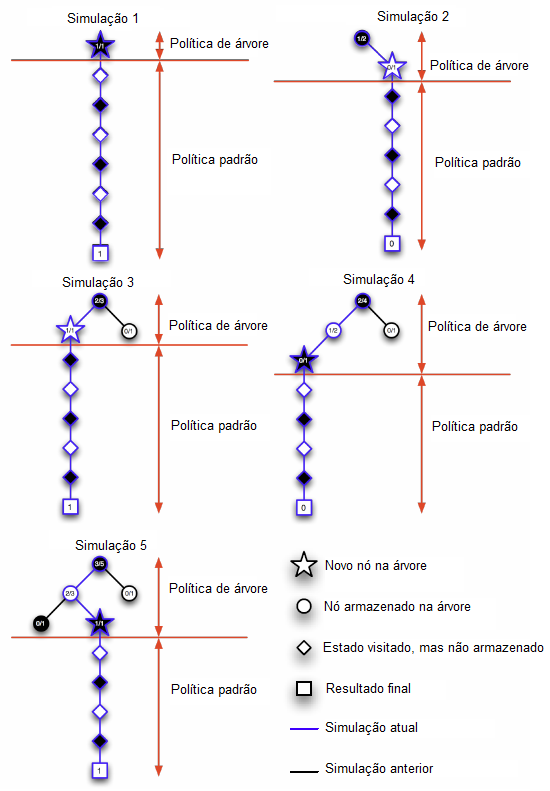
\includegraphics[width=16cm]{figures/politicasMCTS.png}
\caption[Pol�ticas MCTS]{Pol�tica de �rvore e pol�tica padr�o.}
\label{fig:treePolicy}
\end{figure}

Segundo \cite{schadd2009monte} ao finalizar o MCTS existe quatro crit�rios de como escolher o melhor filho:

\begin{itemize}
	
	\item \textbf{Filho m�ximo}: Seleciona o filho com valor mais alto.
	
	\item \textbf{Filho robusto}: Seleciona o filho com o maior n�mero de visitas.
	
	\item \textbf{Filho m�ximo-robusto}: Selecione o filho que tem tanto o maior n�mero de visita e o valor mais alto. Se n�o existir esse filho, � melhor continuar a busca at� achar um filho m�ximo-robusto do que escolher um filho com baixo n�mero de visitas.
	
	\item \textbf{Filho seguro}: Selecione o filho com menor chance de ter resultado negativo.
	
\end{itemize}

\section{Implementa��es MCTS}

A implementa��o mais popular do algoritmo MCTS � o \textit{Upper Confidence Bound for Trees} (UCT) (\cite{browne12asurvey}). Existem outras varia��es como o Online Outcome Sampling (OOS) (\cite{Lanctot2014}) ou utilizando Regret Matching junto com MCTS (\cite{tak2014monte}).	

Diferente dos jogos de turnos tradicionais onde temos turnos sequenciais uniformes, ou seja, primeiro o jogador A depois o B at� que o jogo termine, em batalhas Pok�mon as escolhas s�o feitas simultaneamente e a ordem de execu��o das a��es escolhidas depende de atributos do Pok�mon, da a��o escolhida e outros efeitos especiais. Segundo \cite{tak2014monte} o algoritmo de MCTS que obteve maior sucesso em jogos com turnos simult�neos � o UCT dissociado.

\section{Upper Confidence Bound for Trees (UCT)}

Um dos grandes dilemas na defini��o de pol�tica de �rvore � como balancear as escolhas entre explorar novos n�s para fugir de m�ximos locais e aprofundar de uma sub�rvore existente podendo achar melhores resultados ou garantindo uma maior robustez na avalia��o de um n�. Segundo \cite{auer2002finite} o Upper Confidence Bound for Trees (UCT) resolve essa quest�o de maneira �tima at� um fator constante.

O algoritmo UCT pode ser decomposto em duas partes: MCTS e Upper Confidence Bounds (UCB). Sua primeira implementa��o formal foi em 2006 por Kocsis e Szepesvari \cite{kocsis2006bandit}. O algoritmo UCB entra como uma pol�tica de �rvore para implementa��o de MCTS.


\subsection{Upper Confidence Bounds (UCB)}

O algoritmo mais tradicional de Upper Confidence Bounds � o UCB1 (\cite{auer2002finite}) que foi inicialmente aplicado para o problema \textit{multiarmed bandit}. Segundo \cite{auer2002using} o termo \textit{multiarmed bandit problem} ou problema dos ca�a-n�queis (ou mais precisamente "problema dos K ca�a-n�queis") reflete o problema de um apostador em uma sala com v�rias m�quinas de ca�a n�queis. Em cada tentativa o apostador tem que decidir em qual m�quina ele quer jogar. Para maximizar o ganho total ou recompensa, sua escolha se baseia em recompensas anteriormente coletadas em cada m�quina.

O UCB1 pode ser definido pela seguitne equacao:

\begin{equation}
UCB1 = \overline{x}_{j} + \sqrt{\frac{2 \ln n}{n_{j}}}
\end{equation}

Onde $\overline{x}_{j}$ � a m�dia da recompensa paga pela m�quina $j$, $n_{j}$ � o numero de vezes em que foi jogado na m�quina $j$ e $n$ � a soma de quantas vezes foram em jogadas em todas as m�quinas.

\subsection{Pol�tica de �rvore UCB1}

A aplica��o do UCB1 como pol�tica de �rvore funciona do seguinte modo: no processo de sele��o a escolha pode ser modelada com um problema \textit{multiarmed bandit} independente. A utilizica��o do MCTS com qualquer pol�tica de �rvore UCB � chamada de UCT.

Uma varia��o proposta por \cite{kocsis2006improved} chamada de \textit{plain UCT} provou ter resultados muito superiores ao UCT comum. Ainda segundo \cite{kocsis2006improved} com essa modifica��o a chance de selecionar o melhor movimento  converge em 1 e, atrav�s de testes emp�ricos foi observado que � mais r�pido que outros algoritmos de busca em �rvore como o \textit{alpha-beta}.

A equa��o do \textit{plain UCT} � definida da seguinte forma:

\begin{equation}
UCT = \overline{x}_{j} + 2C_{p} \sqrt{\frac{2 \ln n}{n_{j}}}
\end{equation}

Onde $C_{p} > 0$ � uma constante. O valor � sugerido como $C_{p} = \frac{1}{\sqrt{2}}$ e pode ser ajustado para mais ou menos para regular o n�vel de explora��o.

\subsection{Grupos de Movimentos}

Um aprimoramento para o UCT que foi utilizado neste trabalho � chamado de grupos de movimentos. Proposto por \cite{childs2008transpositions} essa melhoria diminui consideravelmente a quantidade de ramos da �rvore Monte Carlo. A t�cnica consiste em criar uma nova camada onde todas as poss�veis a��es s�o separadas em grupos e o UCB1 � usado para selecionar qual grupo ser� escolhido.

No agente utilizando MCTS foi aplicado nas escolhas dos jogadores. Uma vez que n�o � conhecido quais movimentos o Pok�mon advers�rio tem (cada Pok�mon pode ter apenas 4 golpes dentre dezenas de golpes que cada diferente Pok�mon pode aprender), ficaria muito custoso criar um ramo para cada poss�vel golpe de cada Pok�mon (o Pok�mon da Esp�cie Mew por exemplo, tem dispon�vel mais 120 diferentes movimentos).

Os grupos de movimentos implementados foram os seguintes:

\begin{itemize}
	
	\item \textbf{Grupo A}: Utilizar golpe de dano super efetivo. Um golpe super efetivo � um golpe que recebe um acr�scimo de $ 2 \times$ ou $ 4 \times$ de sua base de ataque de acordo com o tipo do golpe e do tipo do Pok�mon atingido (definido por um sistema de vantagens e desvantagens explicadas no cap�tulo ???).
	
	\item \textbf{Grupo B}: Utilizar outro golpe de dano qualquer.
	
	\item \textbf{Grupo C}: Utilizar golpe de altera��o de estado. Golpe de altera��o de estado podem ser golpes que enfraque�am o inimigo, fortale�a um aliado ou aplique um estado negativo (paralisar, envenenar e etc).
	
	\item \textbf{Grupo D}: Trocar para algum Pok�mon que tenha algum golpe super efetivo (Grupo A) contra o atual inimigo.
	
	\item \textbf{Grupo E}: Trocar para outro Pok�mon qualquer.
	
\end{itemize}

Antes de cada poss�vel golpe ser encaixado em cada grupo � verificado a imunidade do Pok�mon advers�rio a esse golpe. Caso o Pok�mon advers�rio seja imune ou o golpe n�o tenha efeito (como por exemplo, curar quando os pontos de vidas j� est�o 100\%, tentar aplicar o estado de paraliza��o em um Pok�mon j� paralisado, entre outros) o movimento � descartado n�o entrando para nenhum grupo.

Caso um grupo n�o contenha nenhuma a��o o grupo � descartado da fase de sele��o e expans�o do MCTS. No caso de existir mais de uma a��o, a escolha � feita diferente para cada grupo, conforme as seguintes regras:

\begin{itemize}
	
	\item \textbf{Grupo A e B}: � definido por qual golpe tem maior dano bruto (dano antes das redu��es). Definido pela equa��o:
	
	\begin{equation}
		danobruto = efetividade \times stab \times baseforca
	\end{equation}
	
	Onde:
	
		\subitem \textbf{efetividade}: $\frac{1}{4}$ (super n�o efetivo), $\frac{1}{2}$ (n�o efetivo), $1$, $2$ (efetivo) e $4$ (super efetivo).
		
		\subitem \textbf{stab}: $1$ caso o tipo do Pok�mon seja diferente do tipo do golpe e $2$ caso sejam do mesmo tipo.
		
		\subitem \textbf{baseforca}: For�a base do golpe.
	
	\item \textbf{Grupo C}: Escolhido aleatoriamente.
	
	\item \textbf{Grupo D e E}: Maior quantidade de HP e depois a maior quantidade do atributo velocidade.
	
\end{itemize}
	\chapter{Aprendizado de jogos com humanos}
\label{chap:aprendizadoJogosComHumanos}

\section{Introdu��o}

Nesse cap�tulo vamos discutir sobre aprendizagem de m�quina e as tentativas de aprender com humanos. O cap�tulo est� organizado da seguinte forma: primeiro, na se��o \ref{sec:aprendizado} ser� falado sobre aprendizado e, o que isso representa. Na se��o \ref{sec:redesNeurais} ser� apresentado sobre redes neurais. Na se��o \ref{sec:implementacoesRN} � apresentado algumas das principais t�cnicas de redes neurais. Na se��o \ref{sec:neuroevolucao} ser� apresentado o algoritmo de neuroevolu��o. Na se��o \ref{sec:aprendizadoComHumanos} ser� visto como essas t�cnicas s�o aplicadas para aprender contra humanos. Finalmente, na se��o \ref{sec:conclusaoAprendizadoJogosComHumanos}, s�o apresentadas as considera��o finais deste cap�tulo.

\section{Aprendizagem}
\label{sec:aprendizado}

Um dos processos mais naturais e comuns dos seres humanos � o processo de aprender. Segundo \cite{holt2012psychology} existem duas defini��es para aprendizagem que geralmente s�o usadas por psic�logos: "a mudan�a relativamente permanente no comportamento devido � experi�ncia passada" ou, "o processo pelo qual ocorrem mudan�as relativamente permanentes no potencial comportamental como resultado da experi�ncia". J� \cite{de2013learning} afirma que tais defini��es cl�ssicas s�o problem�ticas e define o processo de aprendizado como adapta��o ontogen�tica, ou seja, como mudan�as no comportamento de um organismo resulta de regularidades no ambiente do organismo. Esta defini��o funcional n�o s� resolve os problemas de outras defini��es, mas tamb�m tem importantes vantagens para a pesquisa de aprendizagem cognitiva.

No trabalho de \cite{schunk1996learning}, a aprendizagem, na perspectiva filos�fica, pode ser discutida sob o t�tulo de epistemologia, que se refere ao estudo da origem, natureza, limites e m�todos de conhecimento. Ainda segundo o autor a origem do conhecimento � obtida de dois modos: 

\begin{itemize}

	\item \textbf{Racionalismo}. Refere-se � id�ia de que o conhecimento � derivado da raz�o sem recorrer aos sentidos.
	
	\item \textbf{Empirismo}. No contraste ao racionalismo, o empirismo se refere a ideia que a experi�ncia � a fonte de conhecimento.

\end{itemize}

Fora do campo de psicologia e filosofia pode-se encontrar outras defini��es para o aprendizado, como no trabalho de \cite{carbonell1983overview} que define a aprendizagem como um fen�meno de m�ltiplas faces. O proceso de aprendizado inclue a aquisi��o de novos conhecimentos, o desenvolvimento de habilidades motoras e coginitivas atrav�s de instru��es ou pr�ticas, a organiza��o do conhecimento, e a descoberta de novos fatos e teorias atrav�s da observa��o e experimenta��o.

\subsection{Aprendizado de m�quina}
\label{sec:minimax}

O aprendizado de m�quina s�o modelos matem�ticos para representar o processo de aprendizado com m�quinas, entre outras palavras, o estudo do processo de aprendizado e a modelagem computacional desse processo define o aprendizado de m�quina.

Segundo \cite{carbonell1983overview} o aprendizado de m�quina � organizado em tr�s amplos campos de pesquisa:

\begin{itemize}

	\item \textbf{Estudos orientados a tarefas}. Desenvolvimento e an�lise de sistemas de aprendizado em um predeterminado conjunto de tarefas.
	
	\item \textbf{Simula��o cognitiva}. Investiga��o e simula��o do processo de aprendizado humano.
	
	\item \textbf{An�lise te�rica}. Explora��o te�rica do espa�o dos poss�veis m�todos de aprendizado e algoritmos indenpendentes do dom�nio da aplica��o.

\end{itemize}

%http://stpk.cs.rtu.lv/sites/all/files/stpk/materiali/MI/Artificial%20Intelligence%20A%20Modern%20Approach.pdf%

Segundo \cite{russell1995modern} um agente que utiliza aprendizado de m�quina pode ser descrito pelo seguinte diagrama da \ref{fig:modelLearningAgents}.

\begin{figure}[H]
\centering
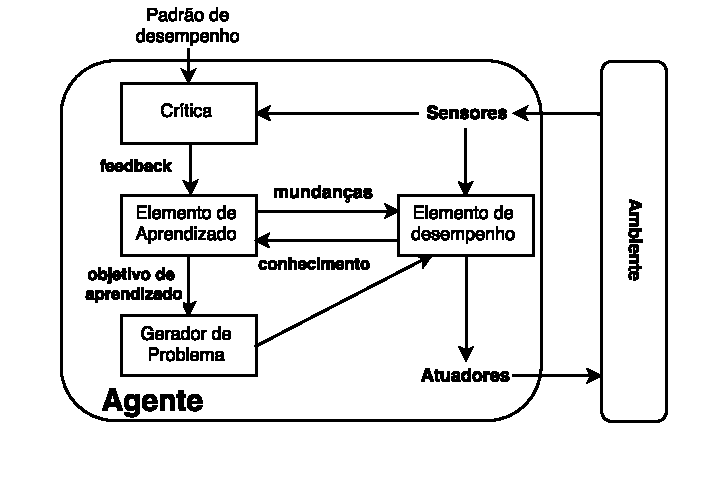
\includegraphics[width=\columnwidth]{figures/modelLearningAgents.pdf}
\caption[Minimax]{\textit{Minimax} aplicado ao Jogo da Velha.}
\label{fig:modelLearningAgents}
\end{figure}

O \textbf{elemento de aprendizado} � respons�vel por ajustar a intelig�ncia do agente. O elemento pega o conhecimento adquirido e um pouco do \textit{feedback} da performance do agente, e determina como o elemento de desempenho dever� ser modificado.

O \textbf{elemento de desempenho} avalia todas as entradas que recebe (sensores, aprendizado e gerador de problema) e escolhe a a��o.

O componente \textbf{cr�tica} avalia qu�o bem o agente est� desempenhando. A cr�tica aplica um padr�o fixo de desempenho, isso � necess�rio porque as pr�prias percep��es n�o fornecem nenhuma indica��o do sucesso do agente.

Por �ltimo, o \textbf{gerador de problema} � respons�vel por sugerir a��es que podem levar a novas experi�ncias que tragam algo novo pro agente. Esse elemento faz com que o agente n�o fique transitando em um pequeno conjunto de a��es julgadas como boas, e avalie outras a��es que n�o foram exploradas ou que foram pouco exploradas.

� muito comum na literatura classificar aprendizado de m�quina de acordo com a avalia��o do \textit{feedback} que o agente faz. As classifica��es s�o:

\begin{itemize}

	\item \textbf{Aprendizagem supervisionada}. Em situa��o onde as entradas e sa�das do componente s�o conhecidas (o elemento que fornece esse mapeamento de sa�da e entrada � chamado de professor).
	
	\item \textbf{Aprendizagem n�o supervisionada}. Situa��o onde a sa�da correta n�o � conhecida .
	
	\item \textbf{Aprendizagem por refor�o}. Nessa abordagem cada a��o escolhida pelo agente recebe um refor�o ou puni��o por�m, sem nunca falar qual � a a��o correta ou a melhor a��o.

\end{itemize}

\section{Redes Neurais}
\label{sec:redesNeurais}

Segundo \cite{koehn1994combining} as redes neurais foram inventadas no esp�rito de ser uma met�fora biol�gica. A met�fora biol�gica para redes neurais � o c�rebro humano. Como o c�rebro, esse modelo computacional consiste em pequenas unidades interconectadas. Essas unidades (ou n�s) t�m habilidades bem simples. Assim, a for�a desse modelo deriva da intera��o dessas unidades. Ela depende da sua estrutura (topologia) e suas conex�es.

Essas pequenas unidades, conex�es e topologias podem ser comparadas a neur�nios e sinapses. Um modelo bem comum e bastante utilizado � o chamado \textit{perceptron}. Segundo \cite{beiu2003survey} uma rede neural de \textit{perceptron} � composta por um grafo onde os n�s s�o neur�nios e as arestas s�o as sinapses. Essa rede tem alguns n�s de entrada, e alguns (ao menos um) n�s de sa�da.

\section{Implementa��es redes neurais}
\label{sec:implementacoesRN}



\section{Neuroevolu��o}
\label{sec:neuroevolucao}



\section{Aprendizado com Humanos}
\label{sec:aprendizadoComHumanos}



\section{Considera��es Finais}
\label{sec:conclusaoAprendizadoJogosComHumanos}



--------------------------------------------------------------------------------------
	\chapter{MCTS para o jogo Pok�mon}
\label{chap:mctsPokemon}

\section{Introdu��o}

Nos cap�tulos anteriores sobre �rvore de jogos e aprendizagem de jogos com humanos. Nesse cap�tulo o foco ser� a implementa��o de um agente para o jogo Pok�mon Showdown!. O interesse em fazer agente para esse jogo s�o quatro fatores. Alto n�vel de competitividade, dezenas de milhares de pessoas jogam diariamente o jogo, al�m da exist�ncia de diversos campeonatos. Jogo de informa��es imperfeitas com grande n�vel de ramifica��o de escolhas. Jogo totalmente \textit{online}, podendo explorar o aprendizado com jogadores humanos num ambiente dif�cil de identificar se o advers�rio � um \textit{bot} ou n�o. Possibilidade de criar uma API para possibilitar outros pesquisadores criar agentes e a possibilidade de se criar uma competi��o entre agentes jogadores.

O cap�tulo est� organizado da seguinte forma: a primeira se��o \ref{sec:pokemon} � apresentada a franquia de jogos Pok�mon. Na pr�xima se��o \ref{sec:batalhaspokemon} � apresentado as mec�nicas e as regras das batalhas Pok�mon. Na se��o \ref{sec:pokemonshowdown} ser� apresentado a plataforma Pok�mon Showdown!, como ela funciona e suas regras competitivas especiais. Na se��o \ref{sec:apipokemonshowdown} ser� apresentado a API para se comunicar com o jogo Pok�monm Showdown!. Em \ref{sec:mctsPokemonShowdown} � mostrado os agentes criados utilizando MCTS para o Pok�mon Showdown!. Finalmente em \ref{sec:experimentosResutlados} o resultados obtidos pelos agentes propostos.

\section{Pok�mon}
\label{sec:pokemon}

\textit{Pocket Monsters} ou Pok�mon � uma s�rie de jogos desenvolvida pela \textit{Game Freak and Creatures Inc.} e publicada pela Nintendo como parte da franquia Pok�mon. O primeiro lan�amento foi em 1996 no Jap�o para o console Game Boy Color, a principal s�rie do jogo � baseada em \textit{Role-Playing-Game} (RPG) e continua a ser lan�ado para consoles port�teis at� hoje (\cite{7336034}).

Ainda segundo \cite{7336034} o objetivo dos jogos de RPG de Pok�mon � capturar monstros chamados de Pok�mon e com eles conseguir ganhar ins�gnias de gin�sios (pr�mio dado por vencer o l�der de gin�sio em uma batalha Pok�mon), para assim ter acesso a liga Pok�mon e se tornar o campe�o dessa (torneio com os melhores treinadores Pok�mon do jogo).

Em 2016 a franquia completou 20 anos desde o lan�amento de seu primeiro jogo. Os �ltimos jogos da franquia principal foram lan�ados no final de 2016 chamados de Pok�mon Sun e Pok�mon Moon.

\subsection{Caracter�sticas de um Pok�mon}

Nos jogos, um Pok�mon � um monstro virtual semelhante a um animal ou objeto com superpoderes. A caracter�stica final do Pok�mon � baseada na caracter�stica de sua esp�cie e de suas caracter�sticas �nicas. Essa combina��o possibilita ter um grande n�vel de customiza��o em cada Pok�mon.

\subsubsection{Esp�cie}

A esp�cie � qual modelo aquele Pok�mon representa. Existem atualmente mais de 800 esp�cies de Pok�mon. Algumas esp�cies podem evoluir para outra esp�cie quando o Pok�mon atinge certos crit�rios. A figura \ref{fig:pokemonespecie} de \cite{pokedex} mostra quatro diferentes esp�cies Pok�mon e suas principais caracter�sticas. Detalhadamente cada esp�cie Pok�mon tem as seguintes caracter�sticas:

\begin{itemize}
	
	\item \textbf{N�mero}. Identifica��o num�rica �nica.
	
	\item \textbf{Nome}. Nome do Pok�mon.
	
	\item \textbf{Tipo}. Cada Pok�mon ter um ou dois tipos associados a sua esp�cie.
	
	\item \textbf{Estat�stica base}. As estat�stica ou atributos base s�o separado em 6 categorias:
		\subitem \textbf{HP ou PS}. Quantidade de pontos de vida Pok�mon;
		\subitem \textbf{Attack ou Ataque}. Quantidade de ataque f�sico do Pok�mon;
		\subitem \textbf{Defense ou Defesa}. Quantidade de defesa f�sica do Pok�mon;
		\subitem \textbf{Special Attack ou Ataque Especial}. Quantidade de ataque m�gico do Pok�mon;
		\subitem \textbf{Special Defense ou Defesa Especial}. Quantidade de defesa m�gica do Pok�mon;
		\subitem \textbf{Speed ou Velocidade}. Quantidade de Velocidade do Pok�mon;
	
	\item \textbf{Gama de habilidades}. Uma esp�cie de Pok�mon tem tr�s habilidades, sendo que o Pok�mon daquela esp�cie ter� apenas uma delas.
	
	\item \textbf{Gama de movimentos}. Uma esp�cie de Pok�mon pode aprender dezenas de golpes diferentes (baseado no tipo e nas caracter�sticas do Pok�mon), sendo que o Pok�mon daquela esp�cie ter� apenas quatro delas.
	
	\item \textbf{Altura base}. Altura base da esp�cie.
	
	\item \textbf{Peso base}. Peso base da esp�cie.
	
	\item \textbf{Sexo}. Algumas esp�cies podem ter apenas um sexo, ou seja, ser apenas macho ou f�mea.
	
\end{itemize}

\begin{figure}[H]
\centering
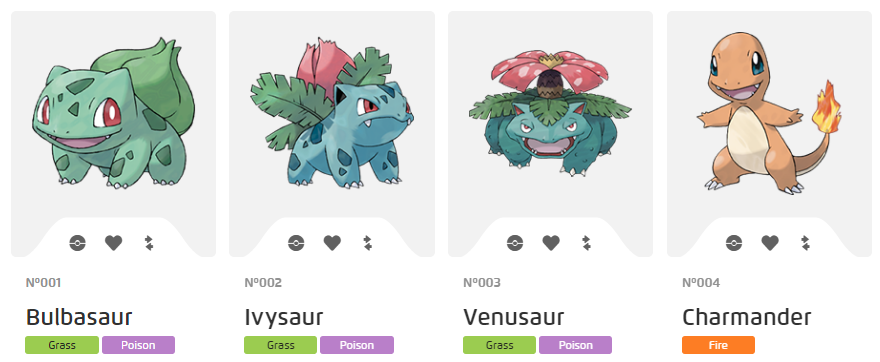
\includegraphics[width=\columnwidth]{figures/pokemonespecie.png}
\caption[Esp�cies Pok�mon]{Esp�cies Pok�mon (\cite{pokedex}).}
\label{fig:pokemonespecie}
\end{figure}

A figura \ref{fig:pokemonmewto} de \cite{pokedex} mostra um exemplo de uma esp�cie Pok�mon e suas caracter�sticas.

\begin{figure}[H]
\centering
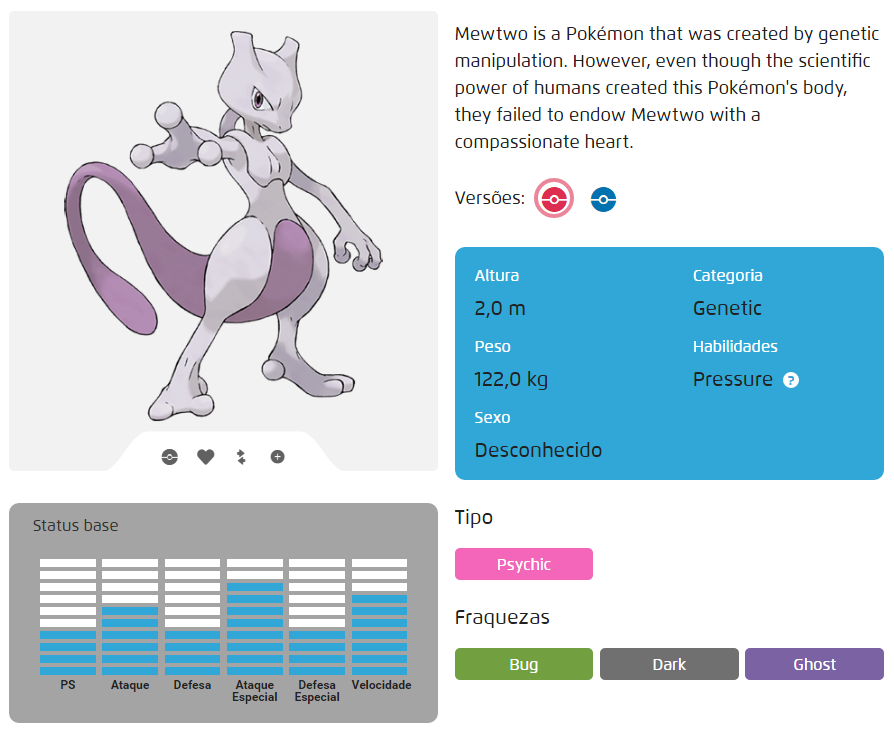
\includegraphics[width=10cm]{figures/pokemonmewto.png}
\caption[Detalhes Pok�mon]{Detalhes Pok�mon Mewtwo (\cite{pokedex}).}
\label{fig:pokemonmewto}
\end{figure}

Existem 18 tipos de Pok�mon entre eles: planta, fogo, �gua, inseto, normal, venenoso, el�trico, terra, lutador, ps�quico, pedra, voador, fantasma, gelo, drag�o, met�lico, noturno e fada.

Alguns tipos de Pok�mon tem vantagem sobre outros tipos de Pok�mon. A ideia � baseada no sistema papel pedra tesoura, onde o papel ganha de pedra, pedra ganha de tesoura e por sua vez tesoura ganha de papel. Por�m no sistema de batalhas Pok�mon essa mec�nica � um pouco mais complexa, uma vez que podem existir at� 2 tipos para cada Pok�mon.

\subsubsection{Caracter�sticas �nicas}

Cada Pok�mon tem uma s�rie de caracter�sticas �nicas, s�o elas:

\begin{itemize}
	
	\item \textbf{Level}. N�vel do Pok�mon. Onde $0 \leq level \leq 100$.
	
	\item \textbf{Effort Values ou EV}. Valores de esfor�o, cada Pok�mon tem 510 pontos de EV que podem ser distribu�dos em qualquer um dos 6 atributos, com a limita��o de que cada atributo pode ter no m�ximo 252 pontos de EV.
	
	\item \textbf{Individual Values ou IV}. Valores individuais, cada atributo do Pok�mon tem um valor de IV associado que varia entre 0 e 31.
	
	\item \textbf{Nature}. Natureza do Pok�mon. Existem 25 diferentes naturezas que um Pok�mon pode ter, sendo que 21 delas alteram atributos. As naturezas que alteram atributos adicionam 10\% em um determinado atributo e reduzem 10\% em outro atributo. A tabela \ref{table:tabelaNatureza} mostra as poss�veis naturezas e as modifica��es dos atributos.
	
\end{itemize}
	
\begin{table}[H]
\centering
\caption{Poss�veis naturezas de um Pok�mon}
\label{table:tabelaNatureza}
\begin{tabular}{|c|c|c|}
\hline
\textbf{Natureza} & \textbf{Atributo aumentado} & \textbf{Atributo diminu�do} \\ \hline
Lonely            & Ataque                      & Defesa                      \\ \hline
Brave             & Ataque                      & Velocidade                  \\ \hline
Adamant           & Ataque                      & Ataque Especial             \\ \hline
Naughty           & Ataque                      & Defesa Especial             \\ \hline
Bold              & Defesa                      & Ataque                      \\ \hline
Relaxed           & Defesa                      & Velocidade                  \\ \hline
Impish            & Defesa                      & Ataque Especial             \\ \hline
Lax               & Defesa                      & Defesa Especial             \\ \hline
Modest            & Ataque Especial             & Ataque                      \\ \hline
Mild              & Ataque Especial             & Defesa                      \\ \hline
Quiet             & Ataque Especial             & Velocidade                  \\ \hline
Rash              & Ataque Especial             & Defesa Especial             \\ \hline
Calm              & Defesa Especial             & Ataque                      \\ \hline
Gentle            & Defesa Especial             & Defesa                      \\ \hline
Sassy             & Defesa Especial             & Velocidade                  \\ \hline
Careful           & Defesa Especial             & Ataque Especial             \\ \hline
Timid             & Velocidade                  & Ataque                      \\ \hline
Hasty             & Velocidade                  & Defesa                      \\ \hline
Jolly             & Velocidade                  & Ataque Especial             \\ \hline
Naive             & Velocidade                  & Defesa Especial             \\ \hline
Hardy             & Nenhum                      & Nenhum                      \\ \hline
Docile            & Nenhum                      & Nenhum                      \\ \hline
Serious           & Nenhum                      & Nenhum                      \\ \hline
Bashful           & Nenhum                      & Nenhum                      \\ \hline
Quirky            & Nenhum                      & Nenhum                      \\ \hline
\end{tabular}
\end{table}

\subsubsection{Caracter�sticas calculadas}

O valor final dos atributos � calculado de duas formas diferentes. O valor final de HP � dado pela seguinte equa��o:

\begin{equation}
V = \Bigg( \frac{ \Big( ( 2 \times Base + IV + \frac{EV}{4} ) \times level \Big) }{100} + level + 10 \Bigg),
\end{equation}

j� o resto dos atributos � dado pela seguinte equa��o:

\begin{equation}
V = \Bigg( \frac{ \Big( ( 2 \times Base + IV + \frac{EV}{4} ) \times level \Big) }{100} + 5 \Bigg) \times Nature,
\end{equation}

onde \textbf{V} � o valor final, valor que o jogador ir� ver no jogo. \textbf{Base} � a quantidade b�sica da estat�stica definido pela esp�cie. \textbf{Nature} Se a natureza do Pok�mon favorecer esse atributo o valor � atribu�do 1.1, caso a natureza desfavore�a esse valor � 0.9 e caso a natureza n�o influa nesse atributo o valor � 1.

Para exemplificar esse c�lculo de atributos mostrar como � importante a customiza��o dentro do jogo do Pok�mon, a seguir ser� calculado o atributo "Especial Ataque"  para 2 Pok�mon da esp�cie Mewtwo ambos no n�vel 100. O Pok�mon Mewtwo tem 154 pontos de Ataque Especial base.

O primeiro Mewtwo ser� chamado de Mewtwo A. O Mewtwo A � da natureza Modest e tem 252 pontos de EV em Ataque Especial e 31 pontos de IV no atributo Ataque Especial. Substituindo essas vari�veis na equa��o:

\begin{equation}
447.7 = \Bigg( \frac{ \Big( ( 2 \times 154 + 31 + \frac{252}{4} ) \times 100 \Big) }{100} + 5 \Bigg) \times 1.1
\end{equation}

O segundo Mewtwo ser� chamado de Mewtwo B. O Mewtwo B � da natureza Adamant e tem 0 pontos de EV em Ataque Especial e 0 pontos de IV no atributo Ataque Especial. Substituindo essas vari�veis na equa��o:

\begin{equation}
281.7 = \Bigg( \frac{ \Big( ( 2 \times 154 + 0 + \frac{0}{4} ) \times 100 \Big) }{100} + 5 \Bigg) \times 0.9
\end{equation}

A diferen�a do atributo Especial Ataque do Mewtwo A e do Mewtwo B � de 166 pontos, ou seja, o Mewtwo A tem cerca de 66\% mais pontos nesse atributo que o Mewtwo B. 

Cada tamb�m Pok�mon pode carregar consigo um item, esse item tamb�m traz certos tipos de benef�cios para o Pok�mon. Alguns itens s�o ativados quando uma condi��o ocorre na batalha, outros itens s�o cont�nuos. Existem cerca de 300 itens diferentes. Um exemplo de item � o \textit{Leftovers} que recupera $\frac{1}{16}$ do HP total do Pok�mon ao final de cada turno.

\section{Batalhas Pok�mon}
\label{sec:batalhaspokemon}

Existem diversos tipos de batalhas dentro do jogo Pok�mon. Nessa se��o � apresentado o modo padr�o de batalha chamado \textit{Single Battle}. Existem outros modos dispon�veis no jogo como:  \textit{Double Batles}, \textit{Tripple Battles} e \textit{Rotation Battle}.

\subsection{Modo Single Battle}
\label{sec:modoShowdown}

As batalhas acontecem em maioria dos momentos do jogo, onde um treinador desafia outro treinador, podendo o vencedor levar um pouco de dinheiro virtual ou uma medalha (tamb�m chamada de ins�gnia).

Cada treinador pode utilizar at� 6 Pok�mon sem quaisquer restri��es. Vence o treinador que desmaiar todos os Pok�mon do advers�rio primeiro, ou seja, quando todos os Pok�mon de um treinador estiverem com o HP igual a zero.

A batalha � realizada por turnos simult�neos. Ao come�ar a batalha ambos os jogadores colocam um Pok�mon no campo de batalha, chamado de Pok�mon ativo. Para ambos os jogadores � mostrado as op��es de golpes e as op��es para trocar de Pok�mon.

A decis�o de quem ir� a executar a a��o primeira ocorre de maneira complexa. Simplificando a ordem de qual a��o acontece primeiro � dado pelo seguinte (n�meros menores mais prioridade):

\begin{itemize}
	
	\item \textbf{1}. A��o de trocar de Pok�mon.
	
	\item \textbf{2}. Golpes de prioridade positiva. Existe um pequeno conjunto de golpes que faz o Pok�mon atacar primeiro independente do crit�rio 3. Se ambos o Pok�mon utilizarem golpes de prioridade o crit�rio 3 decidir� quem realiza a a��o primeiro.
	
	\item \textbf{3}. O Pok�mon com maior atributo de velocidade ataca primeiro.
	
	\item \textbf{4}. Golpes de prioridade negativa. Existe tamb�m um pequeno conjunto de golpes que faz o Pok�mon atacar por �ltimo independente do crit�rio 3. Se ambos o Pok�mon utilizarem golpes de prioridade negativa o crit�rio 3 decidir� quem realiza a a��o primeiro.
	
\end{itemize}

\subsection{Golpes do Pok�mon}
\label{sec:golpesPokemon}

Uma das customiza��es mais importantes s�o quais golpes o Pok�mon ir� poder utilizar. Cada Pok�mon pode escolher 4 golpes entre dezenas de golpes dispon�veis para sua esp�cie. Cada esp�cie de Pok�mon pode aprender um conjunto diferente de habilidades dependendo do seu tipo e caracter�sticas (por exemplo, apenas Pok�mon com chifre conseguem aprender o golpe \textit{Mega Horn}). Existem mais de 600 golpes diferentes.

As principais caracter�sticas dos golpes s�o:

\begin{itemize}

	\item \textbf{Category ou Categoria}. Existem tr�s tipos de categorias:
		
		\subitem \textbf{Status ou Condi��o}. Golpes que n�o infringem dano diretamente, por�m tem algum efeito com grande chance de sucesso para compensar.
		
		\subitem \textbf{Physical ou F�sico}. Golpes f�sicos utilizam o Ataque para c�lculo de dano e Defesa para c�lculo da resist�ncia.
		
		\subitem \textbf{Special ou Especial}. Golpes especiais utilizam o Ataque Especial para c�lculo de dano e Defesa Especial para c�lculo da resist�ncia.

	\item \textbf{Base Power ou For�a base}. A for�a base ou dano base do golpe. Golpes de condi��o n�o tem for�a base
	
	\item \textbf{Tipo}. Se o tipo do golpe (cada golpe tem apenas um tipo) for um dos tipos do Pok�mon que est� usando o golpe a base de for�a � aumentada em 50\% (chamado de STAB ou \textit{Same Type Attack Bonus}).
	
	\item \textbf{Accuracy ou Precis�o}. A chance em percentagem de um golpe acertar.
	
	\item \textbf{PP ou Pontos de Poder}. A quantidade de vezes que um Pok�mon pode usar um 
	golpe durante uma batalha.
	
	\item \textbf{Efeito Secund�rio}. Um golpe pode ter um efeito secund�rio, esse efeito tem uma chance de acontecer e pode afetar uma s�rie de coisas como, por exemplo, deixar o oponente paralisado ou aumentar melhorar algum atributo.
\end{itemize}

� no calculo de dano do golpe que o sistema de papel, pedra e tesoura � aplicado. Existem 6 Situa��es que podem acontecer quando o golpe � utilizado em um Pok�mon:

\begin{itemize}

	\item \textbf{Imune}. O Pok�mon advers�rio � imune ao golpe.

	\item \textbf{N�o muito efetivo}. Quando um golpe \textbf{A} � aplicado a um Pok�mon do tipo \textbf{B} e \textbf{C}, e tanto \textbf{B} quanto \textbf{C} tem vantagem sobre \textbf{A}. Modificador de dano: 0.25.
	
	\item \textbf{N�o efetivo}. Quando um golpe \textbf{A} � aplicado a um Pok�mon do tipo \textbf{B} e \textbf{C}, e \textbf{B} ou \textbf{C} tem vantagem sobre \textbf{A}. Modificador de dano: 0.5.
	
	\item \textbf{Normal}. O golpe n�o tem vantagem ou desvantagem sobre o Pok�mon atingido. Modificador de dano: 1.
	
	\item \textbf{Efetivo}. Quando um golpe \textbf{A} � aplicado a um Pok�mon do tipo \textbf{B} e \textbf{C}, e \textbf{A} tem vantagem sobre \textbf{B} ou \textbf{C}. Modificador de dano: 2.
	
	\item \textbf{Muito efetivo}. Quando um golpe \textbf{A} � aplicado a um Pok�mon do tipo \textbf{B} e \textbf{C}, e \textbf{A} tem vantagem sobre \textbf{B} e \textbf{C}. Modificador de dano: 4.
\end{itemize}

A imagem a seguir foi retirada do site \cite{bulbapedia1} e cont�m uma tabela mostrando o modificador de dano para cada tipo de golpe em rela��o ao tipo do advers�rio. Ao escolher um golpe, o tipo (golpes tem apenas um �nico tipo) desse golpe � confrontado nessa tabela de acordo com o tipo do advers�rio, caso o advers�rio tenha dois tipos a consulta nessa tabela � feita duas vezes e os modificadores s�o multiplicados gerando um modificar final.

\begin{figure}[H]
\centering
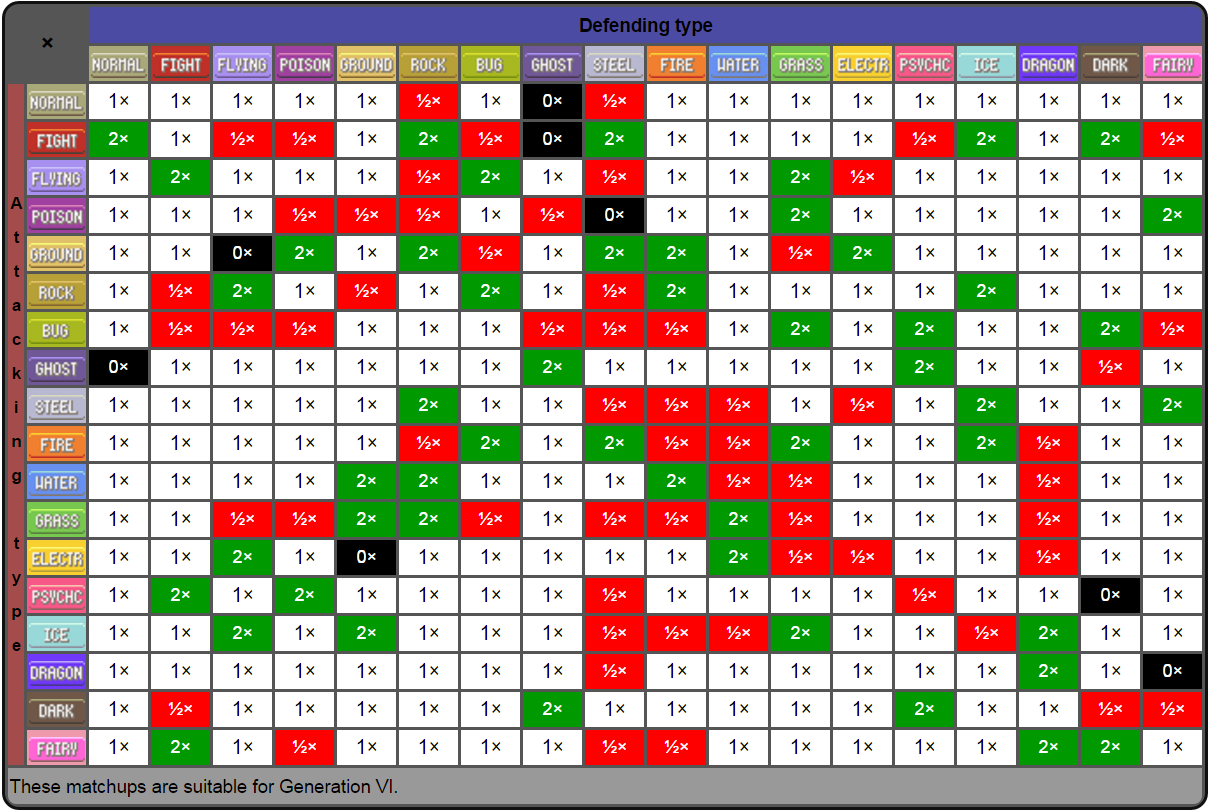
\includegraphics[width=16cm]{figures/pokemontypechart.png}
\caption[Tabela de vantagens e desvantagens do Pok�mon]{Tabela de vantagens e desvantagens do Pok�mon. \cite{bulbapedia1}}
\label{fig:pokemontypechart}
\end{figure}

A equa��o de modificadores de dano � dado por: 

\begin{equation}
Modifier = STAB \times Type \times Critical \times other \times (random[0.85, 1]),
\end{equation}

onde \textbf{Type} � o modificador baseado na vantagem, explicado na subse��o anterior, os valores podem variar entre  0, 0.25, 0.5, 1, 2, e 4. \textbf{Critical} Normalmente um golpe tem chance de cr�tico de 6.25\% caso esse acerto cr�tico ocorra o valor para Critical � de 1.5, caso contr�rio o valor � 1. \textbf{Other} S�o outros modificadores que podem ser adicionados por causa de itens ou estados especiais que modifiquem o dano. \textbf{random} Por final � adicionado um valor aleat�rio entre 85\% e 100\%.

Para calcular a quantidade de HP que um Pok�mon ir� perder ap�s sofrer um golpe � denotado pela seguinte equa��o:

\begin{equation}
Dano = \Bigg( \frac{ 2 \times Level + 10 }{ 250 } \times \frac{Attack}{Defense} \times Base + 2 \Bigg) \times Modifier,
\end{equation}

onde \textbf{Dano}. Quantidade de dano total que o Pok�mon ir� receber. \textbf{Attack}. � quantidade de Ataque caso o golpe seja da categoria f�sico, ou quantidade Ataque Especial caso o golpe seja da categoria especial. \textbf{Defense}. � quantidade de Defesa caso o golpe seja da categoria f�sico, ou quantidade Defesa Especial caso o golpe seja da categoria especial. \textbf{Base}. Base de for�a definido no golpe.

\subsubsection{Estados especiais de batalha}
\label{sssec:estadosEspeciais}

Existem diferentes estados especiais de batalha que um Pok�mon est� sujeito, dentro desses estados existem tr�s tipo: prim�rios, secund�rios e vol�teis. Cada Pok�mon s� pode ser afetado por apenas 1 estado prim�rio de batalha ao mesmo tempo, caso tente ser aplicado mais um estado prim�rio de batalha em um Pok�mon que j� est� sofrendo um estado prim�rio de batalha esse novo estado falhar�. 

Os estados especiais prim�rios de batalhas s�o: 

\begin{itemize}
	\item \textbf{BRN} Estado queimado, nesse estado o Ataque do Pok�mon � reduzido em 50\% e, ao final de cada turno o Pok�mon recebe 12,5\% da vida m�xima como dano.
	\item \textbf{FRZ} Estado congelado, nesse estado o Pok�mon n�o pode utilizar nenhum golpe, a cada turno o Pok�mon tem uma chance de 20\% de se descongelar.
	\item \textbf{PAR} Estado paralisado, nesse estado o Pok�mon tem 25\% de chance de errar seu golpe e, sua velocidade � reduzida para 25\% do valor.
	\item \textbf{PSN} Estado envenenado, nesse estado o Pok�mon perde $\frac{1}{16}$ de seu HP no final do turno, aumentando em $\frac{1}{16}$ para cada turno que ele continuar envenenado.
	\item \textbf{SLP} Estado dormindo, nesse estado o Pok�mon n�o pode atacar. Esse efeito tem dura��o de 1 at� 3 turnos.
\end{itemize}

Existem outras categorias de efeitos que s�o chamados de efeitos secund�rios ou efeitos vol�teis. Diferentemente dos estados prim�rios, um Pok�mon pode ter N desses efeitos aplicados. Existe uma grande lista de efeitos secund�rios. Um efeito secund�rio bastante conhecido � a confus�o, onde o Pok�mon fica confuso de 1 a 4 turnos, caso o Pok�mon esteja confuso ele tem 50\% de chance de bater em si pr�prio ao inv�s de usar o golpe no advers�rio.

\section{Pok�mon Showdown!}
\label{sec:pokemonshowdown}

Pok�mon Showdown � um simulador de batalhas Pok�mon. Permitindo jogar batalhas \textit{online} com times gerados aleatoriamente, times predefinidos, ou construindo seu pr�prio time (\cite{pokemonshowdown1}).

Esse ambiente � totalmente \textit{on-line} e pode ser jogado via navegador de internet. O c�digo fonte do jogo � disponibilizado sobre a licen�a MIT. O projeto � constru�do em Html5, JavaScript 6 e Css3. O dono e principal mantenedor do projeto � Guangcong Luo e todo c�digo fonte do projeto pode ser encontrado no Git Hub.

O ambiente conta um grande n�mero de jogadores simult�neos. Durante o desenvolvimento do trabalho foi verificado que muitas vezes o n�mero de usu�rios simult�neos ultrapassou a quantidade de 12000.

\subsection{Regras especiais Pok�mon Showdown!}
\label{sec:regrasEspeciais}

Competitivamente falando Pok�mon tem uma s�rie de problemas de balanceamento. Diferente dos jogos da franquia principal, o Pok�mon Showdown! aplica algumas restri��es para tornar as batalhas Pok�mon ainda mais competitivas.

Como existem v�rios Pok�mon com atributos muitos mais altos e com movimentos muito melhores que outros algumas regras foram definidas para tornar as batalhas mais justas.

O jogo Pok�mon Showdown! segue as regras definida por uma comunidade de jogadores competitivos chamada Smogon \cite{smogon}, essa comunidade regula e define as regras que s�o utilizadas em cada modo de jogo, para que o jogo se torne mais competitivo e balanceado. Um dos principais trabalhos da Smogon � balancear os mais de 800 Pok�mon distribuindo eles em faixas chamadas de \textit{tiers}. Do mais fraco para o mais forte, os principais \textit{tiers} s�o:

\begin{itemize}
	\item PU;
	\item \textit{Never Used} ou NU;
	\item \textit{Rarely Used} ou RU;
	\item \textit{Under Used} ou UU;
	\item \textit{Over Used} ou OU;
	\item \textit{Ubers}.
\end{itemize}

\subsection{Modos de batalhas Pok�mon Showdown!}

O jogo Pok�mon Showdown! tem algumas dezenas de modos de batalhas diferentes como mostra a imagem
\ref{fig:modobatalhaspokemonshowdown}. Os modos de batalhas s�o altamente influenciados pelas regras da Smogon. Os modos de batalha mais utilizados s�o:

\begin{itemize}

	\item \textbf{Random battle} os dois jogadores s�o pareados com times totalmente aleat�rios. Para balancear esse modo s�o atribu�dos diferentes n�veis de acordo com o \textit{tier} do Pok�mon. Pok�mon NU batalham no n�vel 86, RU 82, UU 78, OU 74 e \textit{Ubers} no n�vel 70. Os Pok�mon do \textit{tier} PU n�o s�o utilizados nesse modo.
	
	\item \textbf{OU Battle} O jogador monta seu time com Pok�mon de no m�ximo \textit{tier} OU e s�o pareados com outro jogador tamb�m com time de Pok�mon de \textit{tier} m�ximo OU. Nesse modo todos Pok�mon batalham no mesmo n�vel.

	\item \textbf{Battle Factory} nesse modo primeiro � sorteado um \textit{tier}, cada jogador recebe um time equilibrado predefinido desse \textit{tier}. Nesse modo todos Pok�mon batalham no mesmo n�vel. Por ser o modo de batalha onde os times dependem menos da sorte � o preferido entre os jogadores profissionais.
	
\end{itemize}

\begin{figure}[H]
\centering
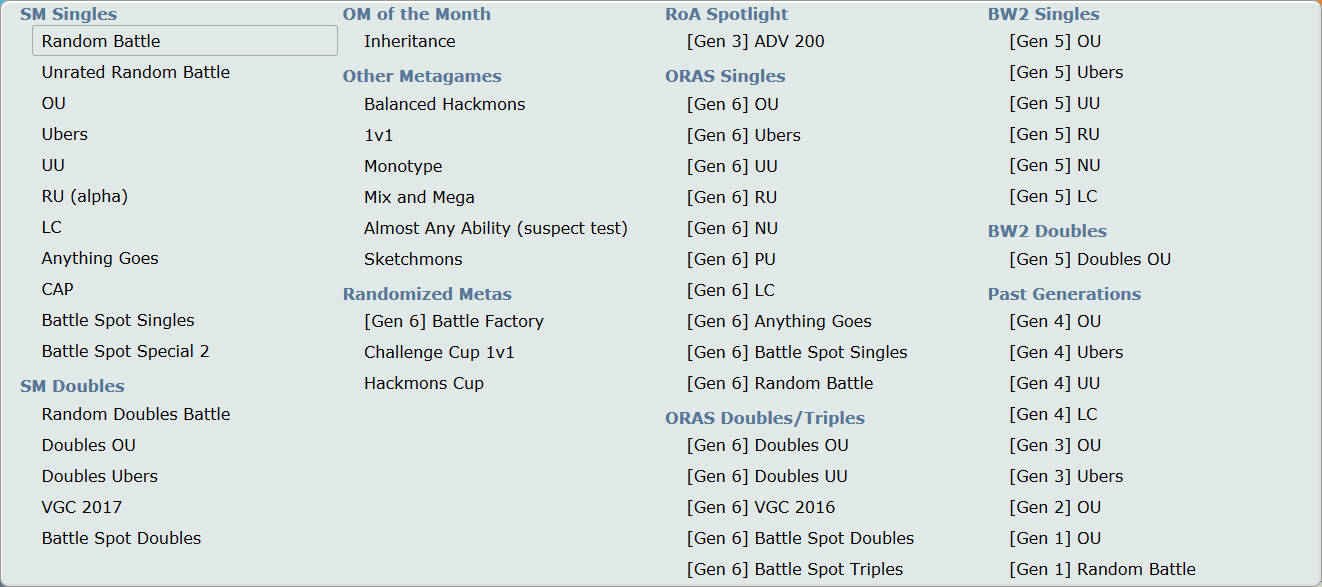
\includegraphics[width=\columnwidth]{figures/modobatalhaspokemonshowdown.png}
\caption[Modos de batalha Pok�mon Showdown!]{Modos de batalha Pok�mon Showdown!.}
\label{fig:modobatalhaspokemonshowdown}
\end{figure}

\subsection{Temporizador de batalha}
\label{sec:temporizadorBatalha}

Todos os modos de jogo do Pok�mon Showdown! contam com um temporizador opcional, ou seja, est� dispon�vel para um dos dois jogadores pedirem para ligar o temporizador. A figura \ref{fig:showdownTimer} mostra a localiza��o do temporizador.

\begin{figure}[H]
\centering
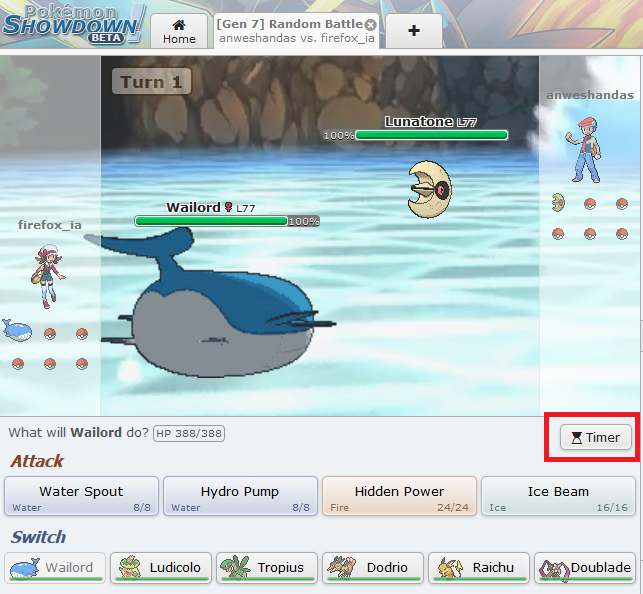
\includegraphics[width=12cm]{figures/showdownTimer.png}
\caption[Bot�o de ligar temporizador de batalha]{Bot�o de ligar temporizador de batalha.}
\label{fig:showdownTimer}
\end{figure}

Uma vez ligado, cada jogador recebe 150 segundos (2 minutos e meio) em seu banco de tempo para ser usado durante toda partida. A cada novo turno cada jogador recebe mais 20 segundos. O jogador que fez a escolha mais r�pida tamb�m ganha 10 segundos adicionais. O tempo m�ximo que se pode ter no banco � de 150 segundos. A figura \ref{fig:showdownTimeLeft} mostra um indicador do tempo restante para realizar sua jogada.

\begin{figure}[H]
\centering
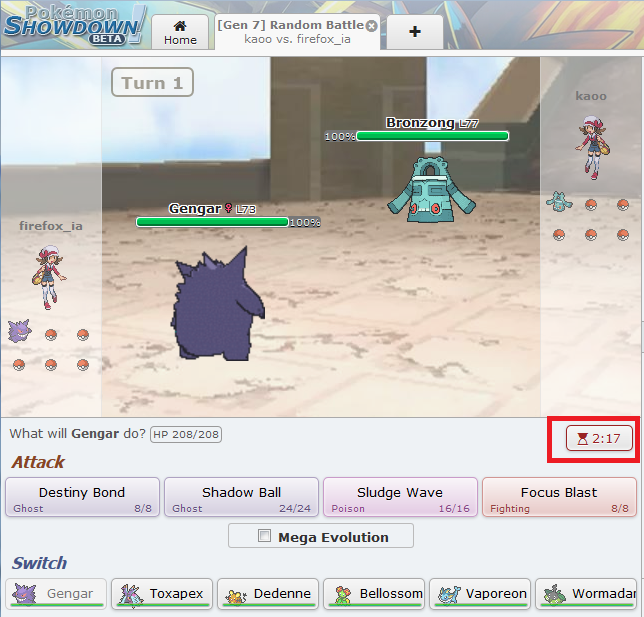
\includegraphics[width=12cm]{figures/showdownTimeLeft.png}
\caption[Quantidade de tempo restante para realizar a jogada]{Quantidade de tempo restante para realizar a jogada.}
\label{fig:showdownTimeLeft}
\end{figure}

\subsection{Sistema de ranqueamento Pok�mon Showdown!}

O Pok�mon Showdown! utiliza o sistema de ranqueamento chamado \textbf{Elo}. O sistema Elo foi criado por Arpad Elo em 1950 como uma evolu��o do sistema de ranqueamento utilizada pela federa��o de xadrez dos Estados Unidos (\cite{glickman1999rating}). Segundo \cite{coulom2007computing} O princ�pio da classifica��o de Elo � que cada jogador recebe uma estimativa de for�a num�rica, calculada a partir da observa��o de resultados do jogo passado.

� muito comum associar Elo a xadrez, por�m muitos jogos digitais, como Pok�mon Showdown!,  e de tabuleiro, como Go, adotam esse mesmo sistema.

Elo tamb�m tem outras fun��es al�m de definir um ranqueamento para um jogador. Ele pode predizer quem tem mais chance de vencer uma partida. Pode ser usado para escolher o advers�rio mais apropriado para um jogo. Segundo \cite{glickman1999rating} o Elo tamb�m � utilizado para definir elegibilidade para torneios e para defini��o de pr�mios.

A pontua��o de Elo de um jogador normalmente varia entre 0 e 3000 que pode ser modificada dependendo do resultado de um campeonato (\cite{coulom2007computing}).

No Pok�mon Showdown! cada jogador tem uma pontua��o de Elo diferente em cada modo de jogo, o sistema de pareamento tenta buscar um advers�rio com semelhante pontua��o de Elo. Cada jogador come�a com 1000 pontos de Elo em todos os modos e, a cada partida, o Elo � atualizado. 

A equa��o para varia��o do Elo ap�s a partida � dado por:

\begin{equation}
V = K \times \Big( score - \frac{ 1 }{ 10^{(foeElo - elo) / 400 } } \Big),
\end{equation}

onde \textbf{V} � a varia��o do Elo. A constante \textbf{K} regula a varia��o do Elo, ou seja, valores grandes para K far� com que cada partida a varia��o de Elo seja maior (para mais e para menos), o Pok�mon Showdown utiliza o valor de K como 50. A vari�vel \textbf{score} resultado da partida, � usado valor 0 para derrotas, 0.5 para empates e 1 para vit�ria. J� \textbf{foeElo} e \textbf{elo} s�o os valores de Elo do advers�rio e seu respectivamente.

Como exemplo, vamos considerar dois jogadores iniciantes chamados \textbf{A} e \textbf{B}. Ambos os jogadores tem 1000 pontos de Elo. Substituindo a equa��o de varia��o do Elo, supondo que o jogador \textbf{A} venceu, se tem:

\begin{equation}
25 = 50 \times \Big( 1 - \frac{ 1 }{ 10^{(1000 - 1000) / 400 } } \Big),
\end{equation}

onde o jogador \textbf{A} totalizaria mais 1025 pontos de Elo.

\section{API para Pok�mon Showdown!}
\label{sec:apipokemonshowdown}

Umas das principais contribui��es desse trabalho � a cria��o de duas APIs para permitir escrever agentes para jogar o Pok�mon Showdown!. A primeira delas � chamada de \textit{showdownAI} e serve como uma camada para facilitar a realiza��o de a��es dentro do jogo. A segunda API � chamada de \textit{showdownSimulation} e sua fun��o � simular em mem�ria uma a��o para poder estimar resultados, essa API � imprescind�vel em algoritmos que precisam prever pr�ximas jogadas como em �rvores de decis�o.

Na imagem \ref{fig:APIsDiagram} mostra como um agente para Pok�mon Showdown! pode trabalhar junto com as APIs, e como elas trabalham com o jogo.

\begin{figure}[H]
\centering
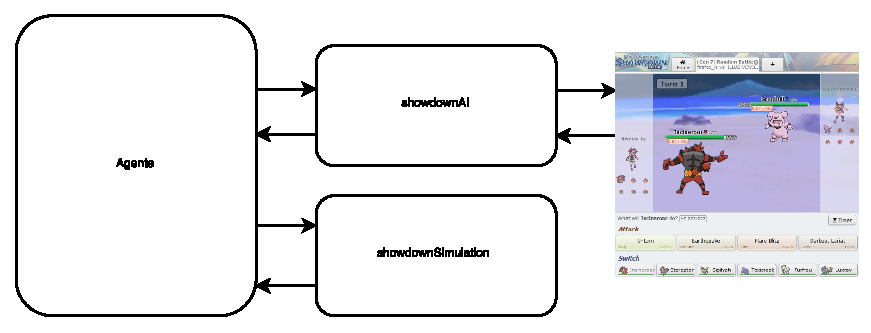
\includegraphics[width=\columnwidth]{figures/APIsDiagram.pdf}
\caption[APIs e Pok�mon Showdown!]{APIs e Pok�mon Showdown!.}
\label{fig:APIsDiagram}
\end{figure}

\subsection{showdownAI}

A API showdownAI � feita em JavaScript e entregue em formato de \textit{plugin} para o Google Chrome para facilitar a instala��o. Todo o c�digo fonte da API � escrito tamb�m e JavaScript. A figura \ref{fig:showdownAIplugin} mostra o \textit{plugin} instalado. 

\begin{figure}[H]
\centering
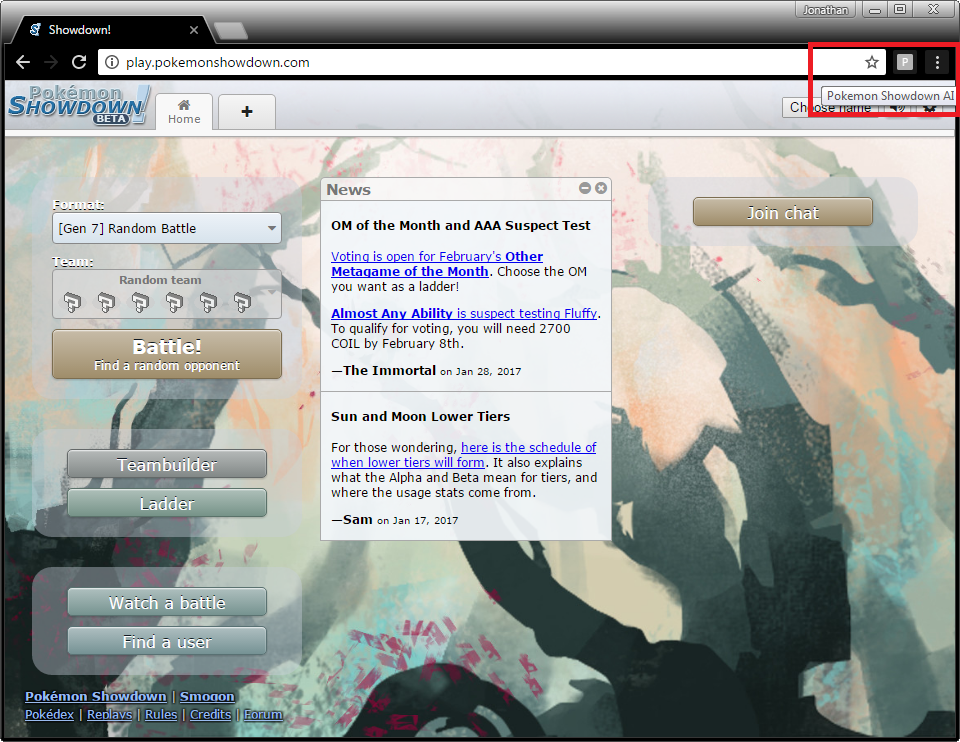
\includegraphics[width=12cm]{figures/showdownAIplugin.png}
\caption[showdownAI \textit{plugin}]{showdownAI \textit{plugin}.}
\label{fig:showdownAIplugin}
\end{figure}

Apesar de ser feito todo em JavaScript, a API showdownAI pode se comunicar com qualquer linguagem que tenha a tecnologia de Sockets atrav�s do recurso de WebSocket (\cite{mdn:websocket}). Com esse recurso o navegador pode se comunicar com um IP (incluindo \textit{localhost}) utilizando Socket.

\subsubsection{M�todos showdownAI}

Os m�todos est�o separados em tr�s blocos: m�todos utilit�rios, m�todos para o menu inicial do jogo (\textit{lobby}) e m�todos para batalhas (\textit{gameplay}). Os m�todos utilit�rios s�o m�todos mais relacionados a API (dados internos), os m�todos para o menu do jogo permitem buscar batalhas e aceitar batalhas e os m�todos de \textit{gameplay} fazem alguma a��o dentro da batalha.

A figura \ref{fig:showdownAIutilityMethods} mostra os m�todos classificados como de utilidade. Com mais detalhes, os principais m�todos s�o:

\begin{itemize}

	\item \textbf{init}. M�todo n�o recebe argumentos nem retorna algum dado. M�todo para inicializar a API.
	
	\item \textbf{log}. M�todo recebe uma mensagem (String) como argumento. Esse m�todo guarda mensagens dentro da API.

	\item \textbf{getLogs}. M�todo retorna um vetor de mensagens (String). Com esse m�todo � poss�vel pegar as mensagens da API.
	
	\item \textbf{getOpponentMessages}. M�todo retorna um vetor de mensagens (String). Com esse m�todo � poss�vel obter as mensagens do \textit{chat} do jogo. O \textit{chat} do jogo � o �nico meio de comunica��o entre os dois jogadores.
	
	\item \textbf{pause}. M�todo n�o recebe argumentos nem retorna algum dado. Esse m�todo faz com que a API para de ler e enviar dados para o Pok�mon Shwodown!.
	
	\item \textbf{pause}. M�todo n�o recebe argumentos nem retorna algum dado. Esse m�todo faz com que a API volte a ler e enviar dados para o Pok�mon Shwodown!.
	
\end{itemize}

\begin{figure}[H]
\centering
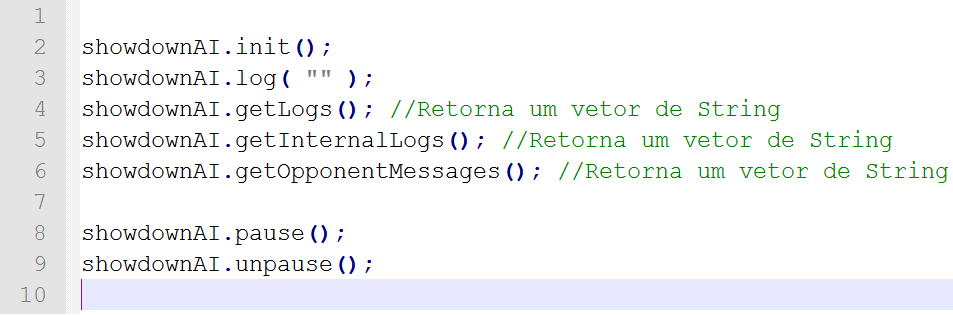
\includegraphics[width=\columnwidth]{figures/showdownAIutilityMethods.png}
\caption[showdownAI m�todos utilit�rios]{showdownAI m�todos utilit�rios.}
\label{fig:showdownAIutilityMethods}
\end{figure}

A figura \ref{fig:showdownAILobbyMethods} mostra os m�todos utilizados no menu inicial. Com mais detalhes, os principais m�todos s�o:

\begin{itemize}

	\item \textbf{login} M�todo recebe como argumento nome do usu�rio, senha e fun��o para ser chamada ap�s o \textit{login} ser efetuado. M�todo n�o cont�m retorno.
	
	\item \textbf{searchRandomBattle}. M�todo recebe como argumento uma fun��o para ser executada ap�s achar uma partida no modo Random Battle. M�todo n�o cont�m retorno.
	
	\item \textbf{searchBattleFactoryBattle}. M�todo recebe como argumento uma fun��o para ser executada ap�s achar uma partida no modo Battle Factory. M�todo n�o cont�m retorno.
	
	\item \textbf{challengeUser}. M�todo recebe como argumento o nome de um usu�rio espec�fico para desafiar e uma fun��o para ser executada quando a batalha come�ar. M�todo n�o cont�m retorno.
	
	\item \textbf{waitForBattleRequest}. M�todo para ficar no menu inicial aceitando qualquer batalha, ele recebe como argumento uma fun��o para ser executada quando a batalha come�ar. M�todo n�o cont�m retorno.
	
\end{itemize}

\begin{figure}[H]
\centering
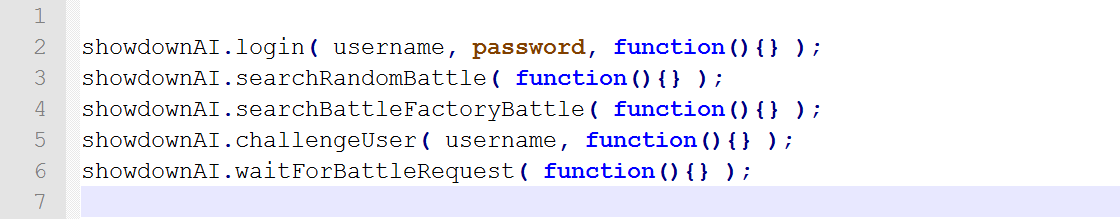
\includegraphics[width=\columnwidth]{figures/showdownAILobbyMethods.png}
\caption[showdownAI m�todos para o menu inicial]{showdownAI m�todos para o menu inicial.}
\label{fig:showdownAILobbyMethods}
\end{figure}

Por fim, a figura \ref{fig:showdownAIBattleMethods1} mostra os m�todos utilizados dentro da batalha. Com mais detalhes, os principais m�todos s�o:

\begin{itemize}

	\item \textbf{getBattleSummary}. M�todo n�o recebe argumentos e retorna um texto com resumo da batalha (nome, quantidade de HP de cada Pok�mon, entre outras informa��es suas e de seu advers�rio ).
	
	\item \textbf{getBattleCommands}. M�todo n�o recebe como argumentos e retorna um objeto do tipo \textit{BattleCommands}. Esse objeto pode conter 3 propriedades/m�tododos:
		
		\subitem \textbf{getStatus}. M�todo que retorna um objeto do tipo \textit{BattleStatus};
		
		\subitem \textbf{result}. Propriedade contendo o resultado da partida (valores poss�veis: WIN, LOST e DRAW);
		
		\subitem \textbf{goToMainMenu}. M�todo que encerra o jogo atual e volta para o menu principal. O m�todo n�o tem argumentos ou retorno.
	
\end{itemize}

\begin{figure}[H]
\centering
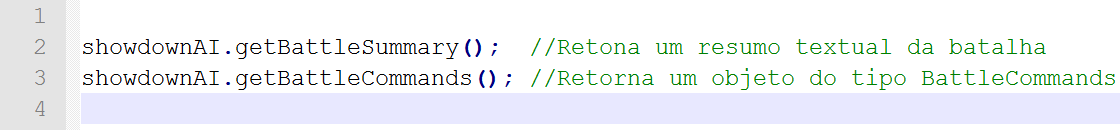
\includegraphics[width=\columnwidth]{figures/showdownAIBattleMethods1.png}
\caption[showdownAI m�todos de batalha parte 1]{showdownAI m�todos de batalha parte 1.}
\label{fig:showdownAIBattleMethods1}
\end{figure}

O objeto \textit{BattleStatus} tem mais 3 grandes objetos dentro dele como mostra a figura \ref{fig:showdownAIBattleMethods2}. As propriedades dele s�o:

\begin{itemize}

	\item \textbf{actions}. Retorna um objeto com os movimentos que o Pokl�mon ativo pode utilizar e os Pok�mon dispon�veis para usar.
	
	\item \textbf{opponent}. Retorna informa��es do advers�rio como: Pok�mon ativo, quantidade restante de Pok�mon. Esse objeto s� retorna informa��es conhecidas sobre o oponente.
	
	\item \textbf{activePokemon}. Retorna um objeto com informa��es do Pok�mon ativo do jogador.
	
\end{itemize}

\begin{figure}[H]
\centering
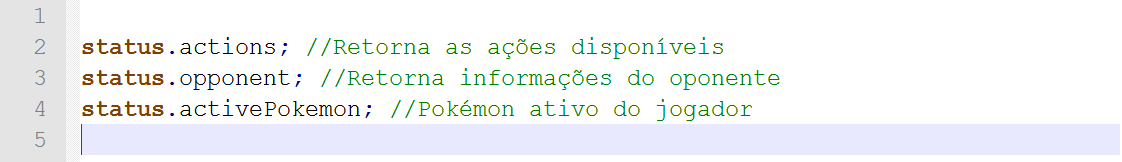
\includegraphics[width=\columnwidth]{figures/showdownAIBattleMethods2.png}
\caption[showdownAI m�todos de batalha parte 2]{showdownAI m�todos de batalha parte 2.}
\label{fig:showdownAIBattleMethods2}
\end{figure}

O objeto \textbf{actions} tem as duas poss�veis a��es do turno, s�o elas: 

\begin{itemize}

	\item \textbf{attacks}. Retorna um vetor com apenas os golpes habilitados. Em cada objeto do vetor existem as seguintes propriedades e m�todos:
		
		\subitem \textbf{name}. Propriedade que retorna o nome do golpe.
		
		\subitem \textbf{info}. Propriedade que retorna informa��es completas do golpe (tipo, dano, entre outros).
		
		\subitem \textbf{use}. M�todo para utilizar o golpe. Esse m�todo recebe como argumento uma fun��o que executar� quando o pr�ximo turno come�ar.
	
	\item \textbf{pokemons}. Retorna um vetor com apenas os Pok�mon que podem entrar na luta. Em cada objeto do vetor existem as seguintes propriedades e m�todos:
		
		\subitem \textbf{name}. Propriedade que o nome do Pok�mon.
		
		\subitem \textbf{info}. Propriedade que retorna informa��es completas do Pok�mon (tipo, atributos, habilidade, item, entre outros).
		
		\subitem \textbf{use}. M�todo para utilizar o Pok�mon. Esse m�todo recebe como argumento uma fun��o que executar� quando o pr�ximo turno come�ar.
	
\end{itemize}

Por fim, o objeto \textbf{opponent} tem todas as informa��es sobre os Pok�mon do advers�rio, as propriedades s�o

\begin{itemize}
	
	\item \textbf{activePokemon}. Retorna um objeto com todas as informa��es conhecidas do Pok�mon ativo do advers�rio.
	
	\item \textbf{activePokemon}. Retorna um vetor de objeto com todas as informa��es conhecidas dos outros Pok�mon.
	
\end{itemize}

\subsubsection{Utilizando showdownAI}

Para exemplificar a utiliza��o da API, na figura \ref{fig:showdownAPISimples} � mostrado um agente para Random Battle que segue os seguintes passos:

\begin{itemize}
	
	\item \textbf{1}. Inicia a API (linha 27) e faz o \textit{login} com uma conta e senha (linha 28).
	
	\item \textbf{2}. Ap�s o \textit{login} acontecer. � chamado o m�todo de buscar batalha no modo Random Battle (linha 29).
	
	\item \textbf{3}. A cada turno se verifica se a partida n�o terminou (linha 2). Se a partida terminou, a partida � finalizada (linha 4), e � buscado novamente uma partida no modo Random Battle (linha 5). Caso n�o tenha terminado, � executado os seguintes sub-passos:
	
		\subitem \textbf{3.1}. Se n�o existe nenhum golpe dispon�vel as a��es poss�veis s�o trocar de Pok�mon (linha 12);
		
		\subitem \textbf{3.2}. Se n�o existe nenhum Pok�mon dispon�vel as a��es poss�veis s�o utilizar um golpe (linha 14);
		
		\subitem \textbf{3.3}. Caso 3.1 e 3.2 n�o aconte�am (linha 16), a��es poss�veis s�o aleatoriamente escolhidas entre utilizar golpes e trocar de Pok�mon (linha 19).
		
		\subitem \textbf{3.4}. Aleatoriamente � escolhido entre as a��es dispon�veis (linha 23).
	
\end{itemize}

\begin{figure}[H]
\centering
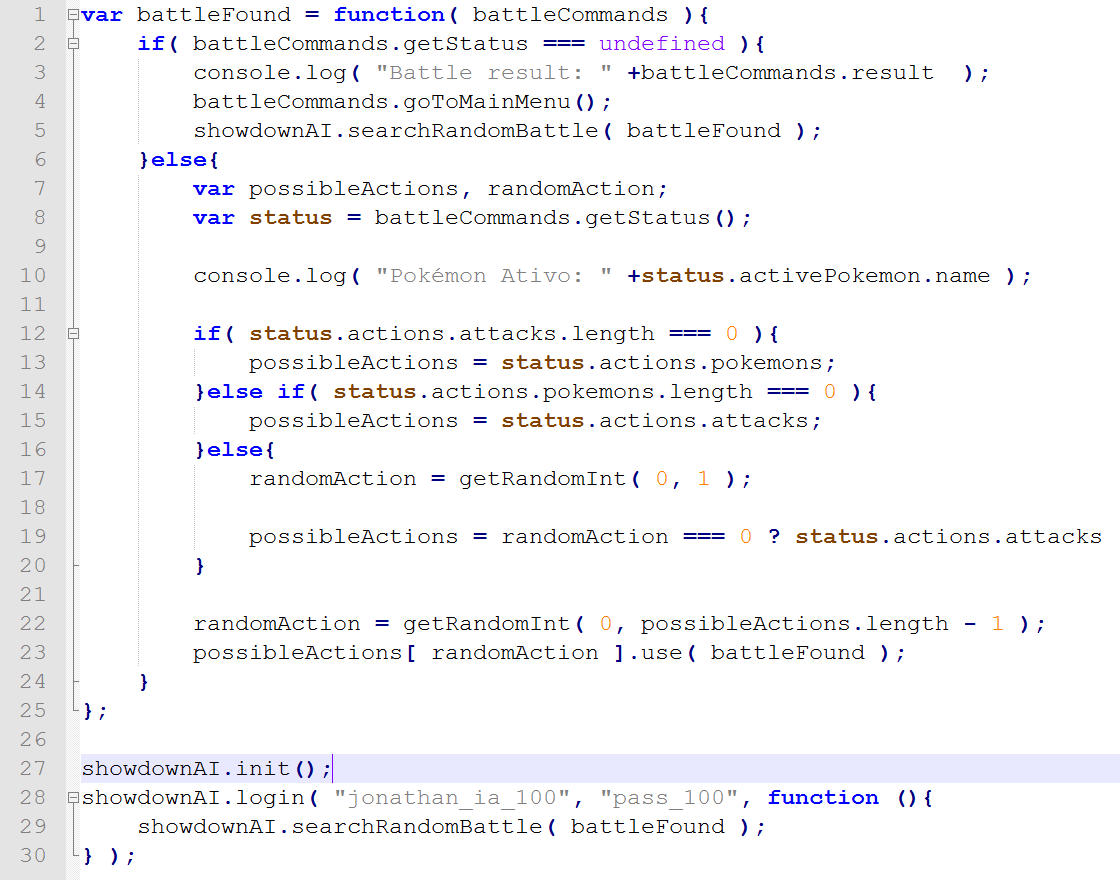
\includegraphics[width=\columnwidth]{figures/showdownAPISimples.png}
\caption[Agente simples utilizando showdownAI]{Agente simples utilizando showdownAI.}
\label{fig:showdownAPISimples}
\end{figure}

\subsection{showdownSimulation}

Em adi��o da API de \textit{gameplay} foi desenvolvido uma API para simular situa��es e, a��es em determinados cen�rios. Isso pode ser feito, pois o c�digo fonte do Pok�mon Showdown! (servidor e cliente) � aberto.

Analisando as classes do c�digo de servidor do Pok�mon Showdown! foi poss�vel isolar o trecho onde s�o criados os times e onde s�o executados as a��es e, com isso, criar a API de simula��o de jogadas.

\subsubsection{Criando uma batalha}

A primeira grande fun��o da API � criar uma batalha completa. A imagem \ref{fig:showdownSimulation1} mostra a utiliza��o da API para criar uma batalha.

\begin{figure}[H]
\centering
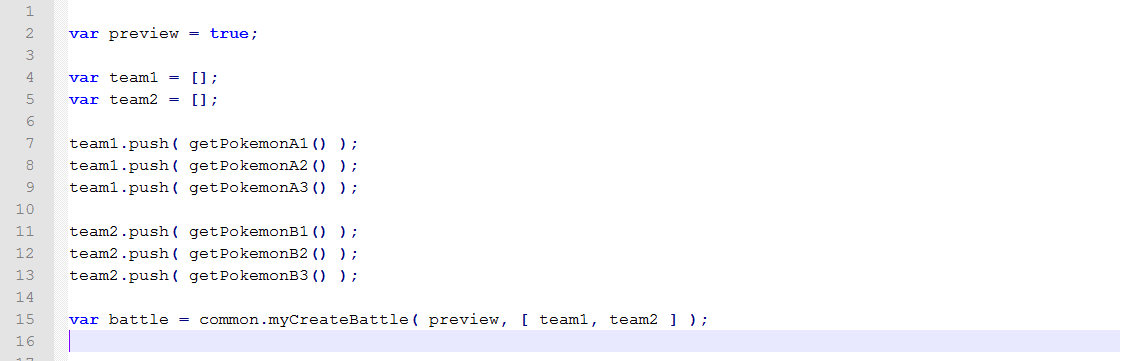
\includegraphics[width=\columnwidth]{figures/showdownSimulation1.png}
\caption[Cria��o de batalha simulada]{Cria��o de batalha simulada.}
\label{fig:showdownSimulation1}
\end{figure}

O m�todo \textbf{myCreateBattle} recebe dois argumentos. O primeiro � chamado de \textbf{preview}, se \textbf{true}, ele define que o primeiro turno da batalha ser� para escolha do Pok�mon inicial, se \textbf{false}, a ordem do vetor do time decidir� qual Pok�mon ir� come�ar na batalha. O segundo argumento � um vetor de times, a primeira posi��o do vetor � o time 1 que � um vetor de objetos Pok�mon, a segunda posi��o do vetor � o time 2 que tamb�m � um vetor de objetos Pok�mon.

N�o � necess�rio um vetor completo de times (seis Pok�mon em cada time) para criar uma batalha, ou seja, � poss�vel simular um jogo onde cada time s� tem um Pok�mon (na imagem \ref{fig:showdownSimulation1} s�o criados dois times com apenas 3 Pok�mon). Tamb�m n�o � necess�rio preencher todos os atributos do objeto Pok�mon para criar uma batalha.

A imagem \ref{fig:showdownSimulation2} mostra dois exemplos de fun��es que criam objetos Pok�mon com todos os atributos para cria��o de batalha.

\begin{figure}[H]
\centering
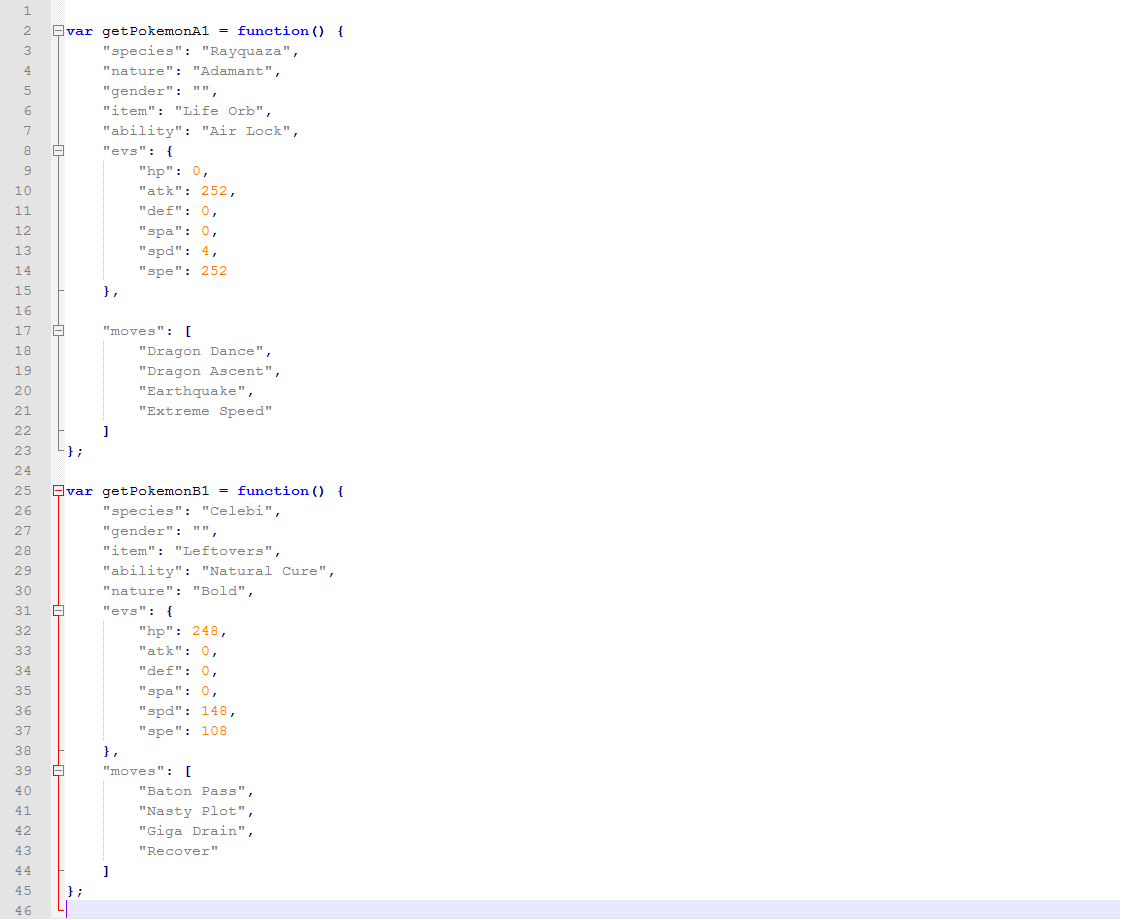
\includegraphics[width=\columnwidth]{figures/showdownSimulation2.png}
\caption[Cria��o de objetos Pok�mon para simula��o]{Cria��o de objetos Pok�mon para simula��o.}
\label{fig:showdownSimulation2}
\end{figure}

O retorno do m�todo \textbf{myCreateBattle} � um objeto chamado \textbf{AITools} com todas as informa��es da batalha que est� sendo simulada. A figura \ref{fig:showdownSimulation3} mostra todos os atributos desse objeto.

\begin{figure}[H]
\centering
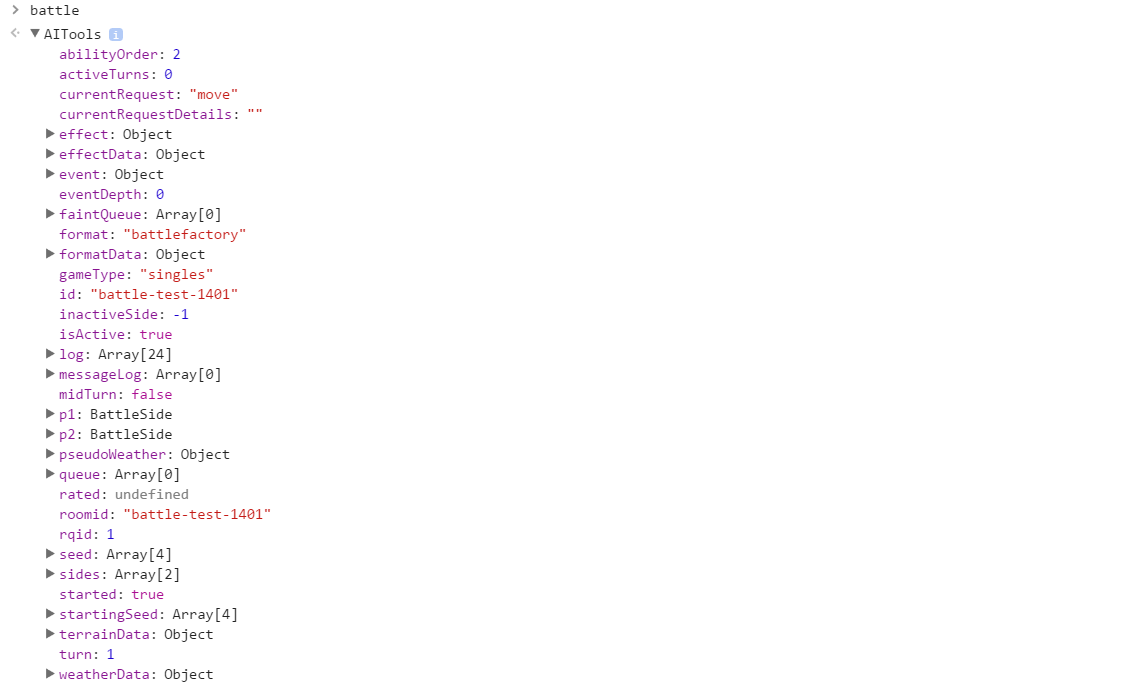
\includegraphics[width=\columnwidth]{figures/showdownSimulation3.png}
\caption[Objeto de simula��o AITools]{Objeto de simula��o AITools.}
\label{fig:showdownSimulation3}
\end{figure}

Os objetos mais importantes dessa classe s�o:

\begin{itemize}
	
	\item \textbf{currentRequest}. � o tipo de turno. Existem tr�s poss�veis valores para essa propriedade:
		
		\subitem \textbf{move}. � o turno padr�o, onde os dois jogadores tem um Pok�mon em campo. Ambos os jogadores podem escolher entre golpes e trocar de Pok�mon.
		
		\subitem \textbf{switch}. � um turno apenas para troca de Pok�mon, normalmente acontece quando um Pok�mon � derrotado e um dos jogadores tem que escolher um novo Pok�mon para entrar em batalha. Alguns golpes tamb�m podem for�ar a troca de Pok�mon, se enquadrando tamb�m nessa situa��o.
		
		\subitem \textbf{teampreview}. Acontece apenas no primeiro turno em batalhas criadas par�metro \textbf{preview} com valor verdadeiro.
	
	\item \textbf{log}. Um vetor de \textit{String} com todas as mensagens do Pok�mon Showdown sobre o que est� acontecendo na simula��o. Informa��es sobre composi��o de cada time, turno atual, movimentos utilizados, entre outras informa��es sobre a batalha est�o dispon�veis nessa propriedade.
	
	\item \textbf{p1} e \textbf{p2}. Objetos com todas as informa��es do jogador1 e jogador2 respectivamente da simula��o.
	
\end{itemize}

Depois de criada a batalha ainda � poss�vel alterar valores do objeto de batalha para melhor refletir a situa��o atual. Algumas propriedades que normalmente s�o necess�rios fazer ajustes: quantidade de HP atual de cada Pok�mon, adicionar estados especiais de batalhas.

\subsubsection{Simulando a��es}

A simula��o de a��es � feita dos objetos \textbf{p1} e \textbf{p2} da batalha simulada. A figura \ref{fig:showdownSimulation4} mostra todos os atributos desse objeto.

\begin{figure}[H]
\centering
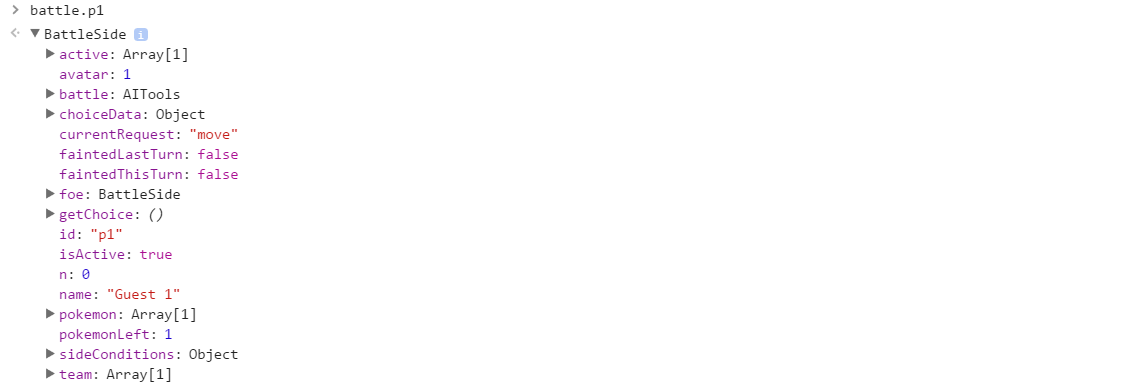
\includegraphics[width=\columnwidth]{figures/showdownSimulation4.png}
\caption[Objetos de simula��o p1 e p2]{Objetos de simula��o p1 e p2.}
\label{fig:showdownSimulation4}
\end{figure}

As propriedades mais importantes dessa classe s�o:

\begin{itemize}

	\item \textbf{active}. Retorna um vetor com os Pok�mon ativos do jogador (como explicado em \ref{sec:batalhaspokemon}, existem lutas de duplas e trios).
	
	\item \textbf{pokemon}. Vetor com todos os Pok�mon dispon�veis e suas informa��es.
	
	\item \textbf{sideConditions}. Alguns golpes podem criar modificadores de terreno (tamb�m chamado de \textit{hazards} de batalha) dando vantagem ou desvantagem ao Pok�mon. Esse objeto cont�m essas informa��es.
	
\end{itemize}

Al�m dessas propriedades, existem tr�s m�todos muito importantes, que fazem as a��es da simula��o:

\begin{itemize}

	\item \textbf{chooseMove}. Esse m�todo recebe como argumento um inteiro com valor de 1 a 4 relacionado ao golpe que o Pok�mon ativo ir� utilizar. Entre outras palavras ao chamar \textbf{chooseMove} passando 1 como argumento, ser� utilizado o golpe de ordem 1 do Pok�mon ativo do jogador.
	
	\item \textbf{chooseSwitch}. Esse m�todo recebe como argumento um inteiro com valor de 1 a 6 relacionado para qual Pok�mon ser� efetuada a troca.
	
	\item \textbf{chooseTeam}. Semelhante ao \textbf{chooseSwitch}, esse m�todo tamb�m recebe como argumento um inteiro com valor de 1 a 6, por�m, esse m�todo s� funciona para o primeiro turno quando existe o \textbf{preview} com valor verdadeiro.
	
\end{itemize}.

A figura \ref{fig:showdownSimulation5} mostra um exemplo de realiza��o de a��es os jogadores. Como a imagem mostra n�o � necess�rio nenhum comando para o turno avan�ar, assim que todos os jogadores fa�am suas escolhas o turno � avan�ado automaticamente. Existem situa��es em que apenas um dos dois jogadores tem que responder como a figura exemplifica.

\begin{figure}[H]
\centering
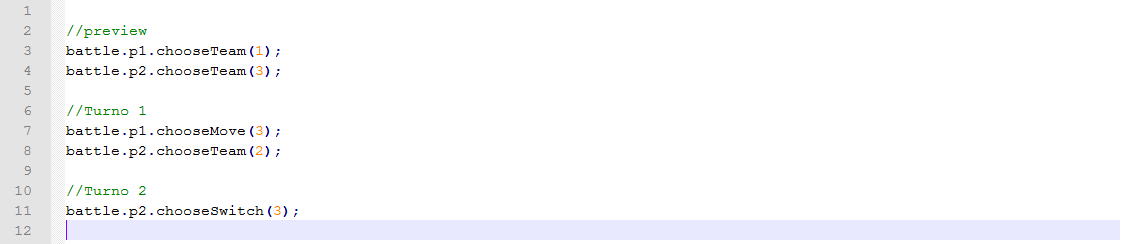
\includegraphics[width=\columnwidth]{figures/showdownSimulation5.png}
\caption[Escolhendo a��es para p1 e p2]{Escolhendo a��es para p1 e p2.}
\label{fig:showdownSimulation5}
\end{figure}

\section{Agentes MCTS para Pok�mon}
\label{sec:mctsPokemonShowdown}

Utilizando as APIs desenvolvidas foram criados 4 agentes para testar os diferentes modos de jogo e validar algumas t�cnicas. Foram criados 2 agentes para \textbf{Random Battle} e 2 agentes para \textbf{Battle Factory}. Nesta se��o ser�o mostradas as t�cnicas utilizadas em cada agente e como ele foi empregado para o problema proposto.

Nos 4 agentes foram utilizadas t�cnicas de MCTS (explicados em \ref{sec:MCTS}), em alguns casos com modifica��es para se adequar ao teste proposto.

\subsection{Agentes para Random Battle}

Nesses dois primeiros agentes foram utilizados apenas a \textbf{showdownAI}, ou seja, n�o foram utilizados elementos de simula��o durante o algoritmo. A ideia desses agentes � descobrir qual tipo de jogadas os agentes priorizam em certos momentos da batalha, ou seja, sem ter conhecimento nenhum sobre o jogo, descobrir em cada turno que se passa se � melhor utilizar: golpes fortes, golpes com efeitos de altera��o de estados, trocar de Pok�mon, entre outros. 

Para realizar esse aprendizado, cada agente conta com dois modos: modo de aprendizagem e modo competitivo. No modo aprendizado os agentes escolhem sempre o grupo de a��es menos explorado. No modo competitivo ele utiliza a base de dados estabelecida na fase de treino para escolher a melhor a��o poss�vel, por�m, ainda alimentando a base de dados.

Ambos os agentes utilizam a mesmo algoritmo. A �nica diferen�a entre os dois um dos agentes � que um dos agentes efetua o treinamento contra humanos (o agente ser� chamado \textbf{humanRandomAgent} ) e o outro contra um terceiro agente c�pia desse agente no modo competitivo (o agente ser� chamado \textbf{botRandomAgent} ).

\subsubsection{Implementa��o dos agentes para Random Battle}

Para diminuir a largura da �rvore de decis�es e adicionar algum conhecimento de jogo durante as escolhas foi utilizada a t�cnicas de Grupos de Movimentos (detalhada em \ref{sec:GruposMovimentos}). 

Em um turno comum cada jogador tem no m�ximo 9 escolhas: escolher um dos 4 golpes ou trocar para um dos outros 5 Pok�mon. Essas escolhas foram classificadas em 5 grupos. Em grande maioria das vezes apenas 2 ou 3 grupos tinha alguma a��o, diminuindo ainda mais a largura da �rvore, os grupos est�o divididos do seguinte modo:

\begin{itemize}

	\item \textbf{Grupo A}. Golpe que s�o efetivos ou muito efetivos (\ref{sec:golpesPokemon}) contra o Pok�mon advers�rio.
	
	\item \textbf{Grupo B}. Golpes de condi��o, ou seja, golpes que alteram algum estado do advers�rio ou pode trazer alguma vantagem para o jogador.
	
	\item \textbf{Grupo C}. Golpes restantes que n�o se encaixam no Grupo A ou no Grupo B.
	
	
	\item \textbf{Grupo D}. Trocar para um Pok�mon que o tipo dele tenha vantagem contra os tipos do Pok�mon advers�rio atual.
	
	\item \textbf{Grupo E}. Trocar para outro Pok�mon que n�o se adequa ao Grupo D.
	
\end{itemize}.

O pseudoc�digo \ref{alg:mctsGruposMovimento} mostra como s�o criados os grupos.

\begin{algorithm}[H]
\caption{Algoritmo de cria��o de grupos}
\label{alg:mctsGruposMovimento}
\begin{algorithmic}[1]
\Procedure{CreateGroups}{$activePokemon, myPokemonList, oponnentPokemon$}
	\State $groups\gets []$
	\State
	\State $groupA\gets []$
	\State $groupB\gets []$
	\State $groupC\gets []$
	\State $groupD\gets []$
	\State $groupE\gets []$
	\State
	\State $weakAndResist\gets \Call{getWeaknessAndResistances}{oponnentPokemon}$
	\State
	\State $groupA\gets \Call{getEffectivenessMoves}{activePokemon, weakAndResist}$
	\State $groupB\gets \Call{getStatusMoves}{activePokemon}$
	\State $groupC\gets \Call{getOtherMoves}{activePokemon, groupA}$
	
	\State $groupD\gets \Call{getEffectivenessPokemon}{myPokemonList, weakAndResist}$
	\State $groupE\gets \Call{getOtherMoves}{myPokemonList, groupD}$
	\State
	\State $groups\gets \Call{addAll}{groupA, groupB, groupC, groupD, groupE}$
\EndProcedure
\end{algorithmic}
\end{algorithm}

A fun��o \textbf{getWeaknessAndResistances} tamb�m faz parte tamb�m da API showdownAI. A imagem \ref{fig:weaknessResist} mostra a utiliza��o dela. Como a figura mostra n�o � necess�rio o preenchimento completo do objeto Pok�mon, basta passar os tipos a serem analisados.

\begin{figure}[H]
\centering
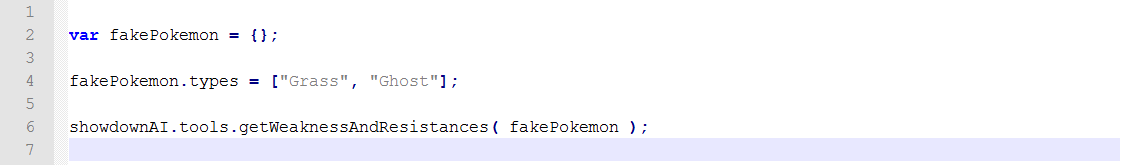
\includegraphics[width=\columnwidth]{figures/weaknessResist.png}
\caption[M�todo getWeaknessAndResistances da showdownAI]{Utiliza��o do m�todo getWeaknessAndResistances da showdownAI.}
\label{fig:weaknessResist}
\end{figure}

A figura \ref{fig:weaknessResistResult} mostra o objeto de retorno do m�todo \textbf{getWeaknessAndResistances}. Como mostra a imagem � retornado um objeto com 5 vetores de \textbf{String} representando: imunidades (tipo de golpe que � imune ao Pok�mon), super resist�ncias (tipo de golpe que � n�o muito efetivo ao Pok�mon), resist�ncias (tipo de golpe que � n�o efetivo), fraquezas (tipo de golpe que � efetivo ao Pok�mon) e super fraqueza (tipo de golpe que � muito efetivo ao Pok�mon).

\begin{figure}[H]
\centering
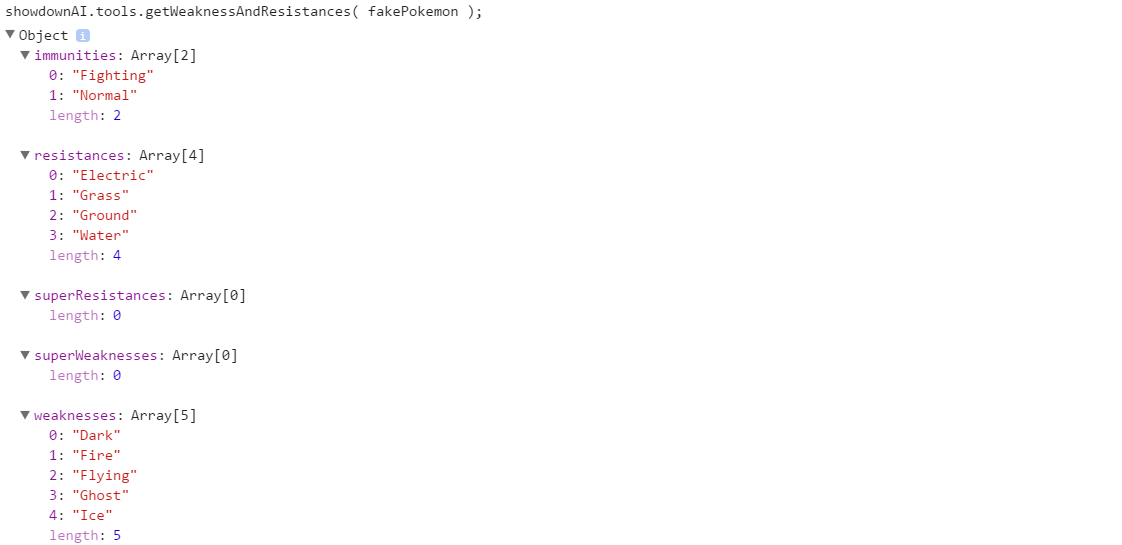
\includegraphics[width=\columnwidth]{figures/weaknessResistResult.png}
\caption[Objeto resultado do m�todo getWeaknessAndResistances]{Objeto resultado do m�todo getWeaknessAndResistances.}
\label{fig:weaknessResistResult}
\end{figure}

O algoritmo utilizado pelos dois agentes foi o UCT descrito em \ref{sec:uct}. A simula��o � feita na base de dados gerada pelo agente. No modo treino a �nica diferen�a do UCT era a fase de sele��o durante o modo treino, que era sempre escolhido o grupo menos testado.

\subsubsection{Implementa��o dos agentes para Battle Factory}

Nos outros dois agentes foi utilizado tanto a API \textbf{showdownAI} quanto a API \textbf{showdownSimulation}. Em um dos agentes foi utilizado um algoritmo comum de MCTS e no outro agente foi utilizada uma vers�o do MCTS para jogos simult�neos. 

A ideia de cria��o dos dois algoritmos � ver a diferen�a de desempenho entre eles. Por isso foi utilizado o modo \textit{Battle Factory} que, competitivamente falando, s�o modos menos aleat�rios.

Nesses agentes foram adicionados alguns conhecimentos sobre o jogo. Al�m de criar simula��es, a API \textbf{showdownSimulation} tem uma base de dados com as principais constru��es de cada Pok�mon, ou seja, nela tem informa��es sobre as customiza��es mais utilizadas para aquele Pok�mon como: golpes mais utilizados, itens, habilidades e distribui��o de EV. Isso � feito atrav�s do objeto p�blico \textbf{factory}. 

O objeto \textbf{factory} est� separado por \textit{tiers} (descritos na se��o: \ref{sec:regrasEspeciais}) como mostra a imagem \ref{fig:factoryTier}.

\begin{figure}[H]
\centering
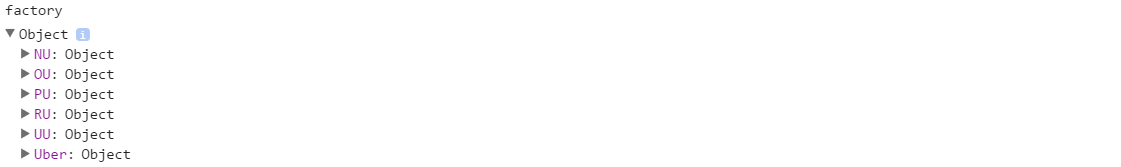
\includegraphics[width=\columnwidth]{figures/factoryTier.png}
\caption[Objeto factory da showdownSimulation]{Objeto factory da showdownSimulation.}
\label{fig:factoryTier}
\end{figure}

Em cada \textit{tier} tem dispon�vel todos Pok�mon e, em cada Pok�mon tem as customiza��es mais usadas (chamadas de \textit{sets}). Na imagem \ref{fig:factoryPokemon} mostra um exemplo dos \textit{sets} para o Pok�mon Mewtwo.

\begin{figure}[H]
\centering
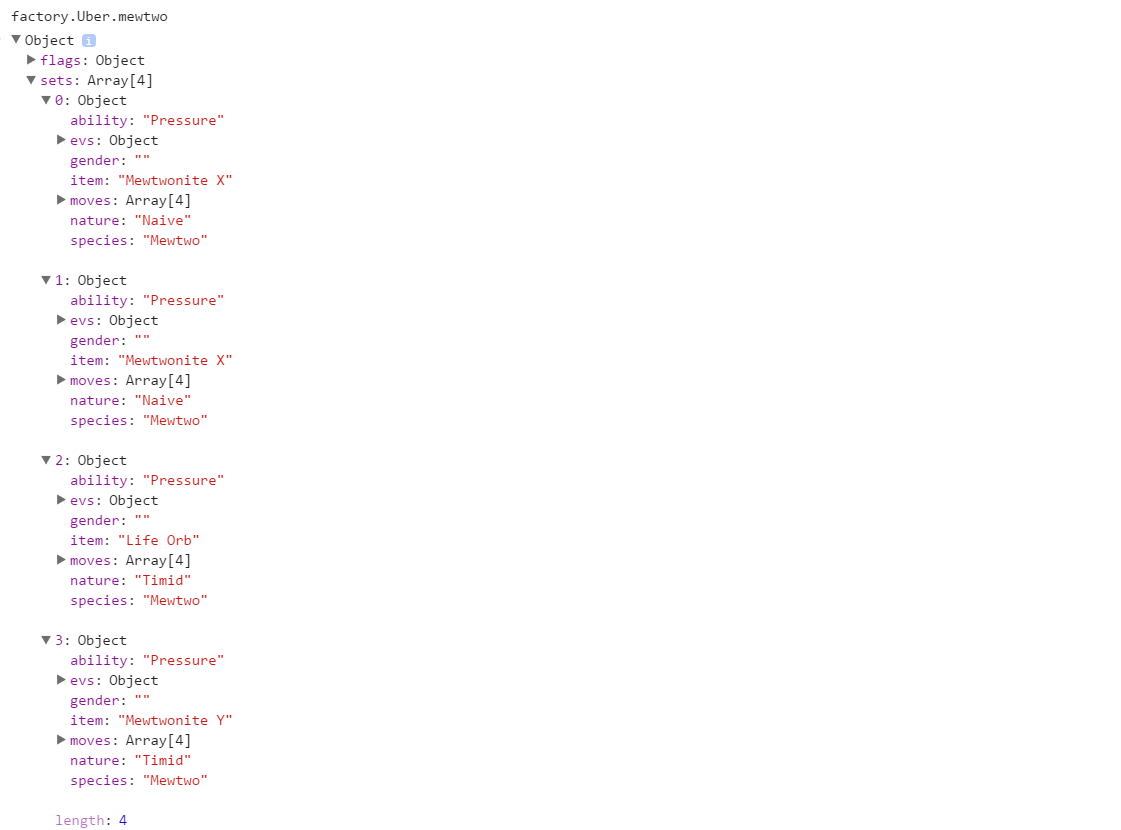
\includegraphics[width=\columnwidth]{figures/factoryPokemon.png}
\caption[Sets de um determinado Pok�mon]{Sets de um determinado Pok�mon.}
\label{fig:factoryPokemon}
\end{figure}

O objeto \textbf{factory} � muito importante nesses agentes, uma vez que n�o � conhecida qual customiza��o o advers�rio utilizou em cada Pok�mon, com um pouco de informa��o sobre o Pok�mon j� � poss�vel estimar qual customiza��o foi utilizada. Entre outras palavras, para fazer a simula��o � pego todas as informa��es que s�o conhecidas durante a batalha sobre aquele Pok�mon e � escolhido o \textit{set} que mais se assemelha a essas informa��es.

\subsubsection{Implementa��o dos agentes para Battle Factory}

O primeiro agente utiliza o algoritmo DUCT (exposto em \ref{sec:duct}) esse agente � chamado de \textbf{ductAgent}. O outro utiliza UCT sem modifica��es chamado de \textbf{uctAgent}.

Com a API de simula��o n�o existe nenhuma base de dados de treinamento, ou seja, cada jogada � simulada em mem�ria e a simula��o � feita at� o fim de jogo (como o algoritmo de MCTS define).

Os dois agentes fazem os 4 passos do MCTS (sele��o, expans�o, simula��o e retropropaga��o) enquanto o temporizador de batalha tenha mais de 30 segundos. Desse modo os primeiros turnos de jogo, onde a altura da �rvore e largura � muito maior, o agente tem 2 minutos para processar e, no decorrer dos demais turnos o agente tem entre 20 e 30 para estimar a melhor jogada (a quantidade de tempo ganha por turno � detalhada em \ref{sec:temporizadorBatalha}).

Cada n� da �rvore de busca cont�m uma c�pia da batalha inteira. Para isso, toda vez que um n� � criado (fase de expans�o do MCTS) � feito uma c�pia completa do time dos dois jogadores. 

A c�pia dos times � feita pela \textbf{showdownSimulation} como a imagem \ref{fig:createCurrentSimulation}. 

\begin{figure}[H]
\centering
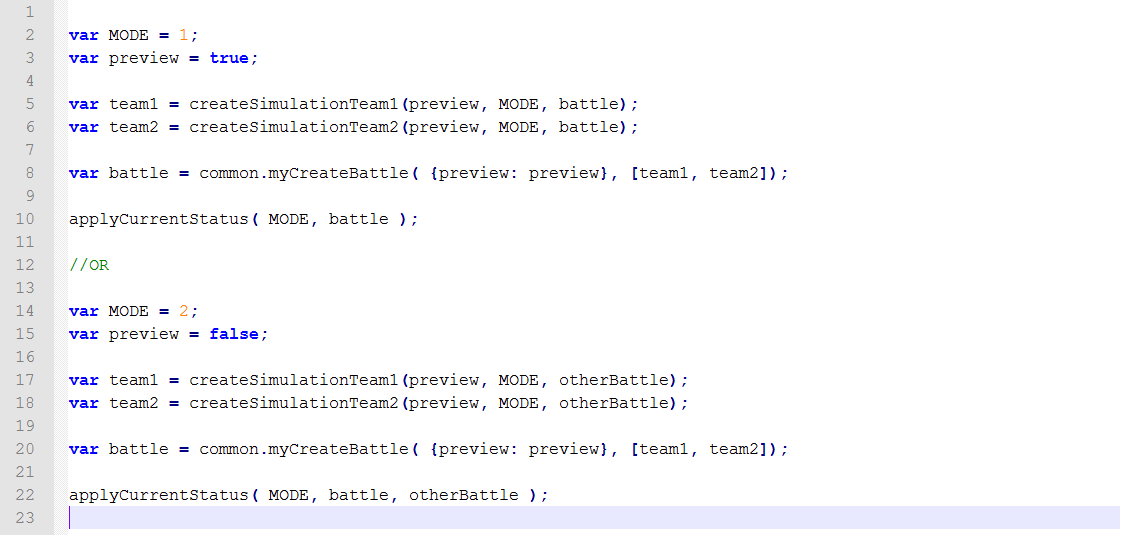
\includegraphics[width=\columnwidth]{figures/createCurrentSimulation.png}
\caption[Criando uma c�pia da batalha]{Criando uma c�pia da batalha.}
\label{fig:createCurrentSimulation}
\end{figure}

Os m�todos \textbf{createSimulationTeam1}, \textbf{createSimulationTeam2} e \textbf{applyCurrentStatus} est�o todos na API \textbf{showdownSimulation}. O m�todo \textbf{createSimulationTeam1} e \textbf{createSimulationTeam2} criam uma c�pia dos times dos jogadores 1 e 2 respectivamente, j� o m�todo \textbf{applyCurrentStatus} � utilizado ap�s o m�todo \textbf{myCreateBattle} para aplicar a situa��o atual de cada Pok�mon. Na figura \ref{fig:createCurrentSimulation} � mostrado dois modos diferente de como utilizar esses m�todos. No primeiro modo (linha 2 at� linha 10) � criado uma c�pia do estado atual da batalha, ou seja, da que est� acontecendo no navegador, para isso a API \textbf{showdownSimulation} utiliza a API \textbf{showdownAI}. No segundo modo (linha 14 at� linha 22) � necess�rio passar mais um argumento para os m�todos que � uma batalha simulada, ou seja, quando um n� diferente do n� raiz � expandido, esse modo � utilizado.

A figura \ref{fig:ductRootNode} mostra o estado do n� raiz do agente \textbf{ductAgent} ap�s 414 passos do DUCT.

\begin{figure}[H]
\centering
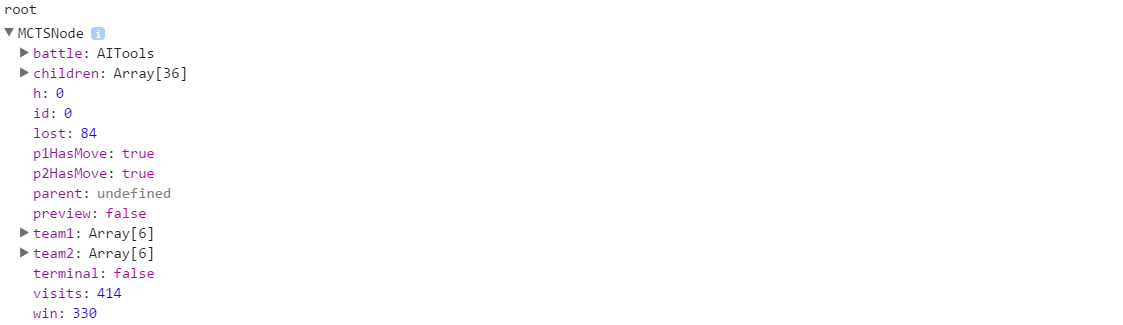
\includegraphics[width=\columnwidth]{figures/ductRootNode.png}
\caption[N� raiz DUCT]{Estado do n� raiz ap�s 414 passos utilizando DUCT.}
\label{fig:ductRootNode}
\end{figure}

\section{Experimentos e Resultados}
\label{sec:experimentosResutlados}
	\chapter{Conclus�es e pesquisas futuras}
\label{chap:conclusoesPesquisasFuturas}

\section{Introdu��o}


\section{Tomada de decis�o}
\label{sec:tomadaDecisao}


	\bibliographystyle{apalike}	
	\bibliography{Bibliografia}

\end{document}